\chapter{Le Modèle Standard} \label{chap:sm}

\begin{fmffile}{chapitre1}

\section{Les particules élémentaires}

La Nature semble avoir décidé de construire la matière à l'aide d'un petit nombre de briques fondamentales, les particules élémentaires. Le Modèle Standard est notre tentative de décrire les interactions entre ces particules. En développement depuis le début du XXe siècle, ce modèle permet maintenant de reproduire avec une précision remarquable les observations expérimentales.

La Nature est ainsi constituée de trois classes de particules élémentaires : les quarks, les leptons et les bosons. Ces particules se déplacent à des vitesses proche de la vitesse de la lumière. Le formalisme mathématique utilisé pour décrire ces particules est la théorie quantique des champs, qui incorpore la mécanique quantique et la relativité restreinte.

Les quarks et les leptons, constituants élémentaires de la matière, sont des particules élémentaires de spin 1/2 : ensemble, ils forment les fermions. Les bosons sont eux de spin entier, et sont les médiateurs des différentes interactions entre les fermions. La figure \ref{fig:sm} liste les particules élémentaires, dans l'état actuel de nos connaissances.

\begin{figure} \centering
  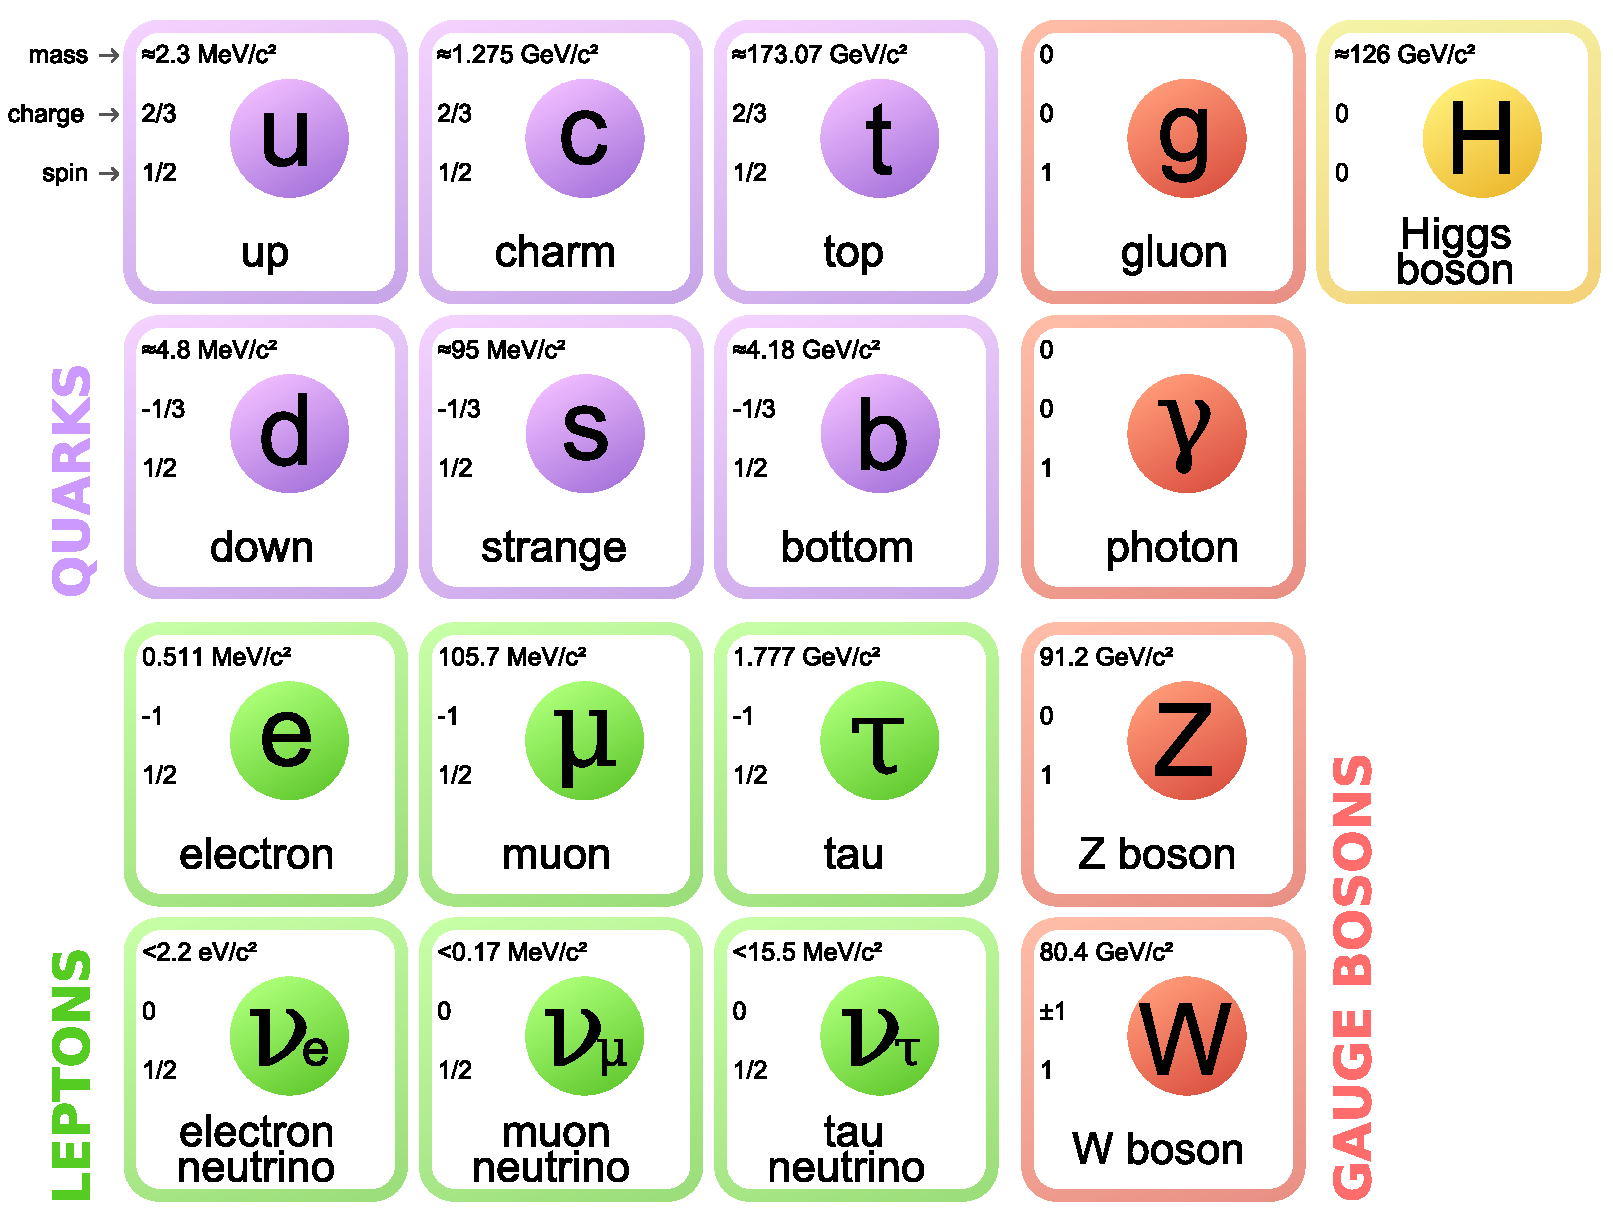
\includegraphics[height=0.4\textwidth]{Standard_Model_of_Elementary_Particles.pdf}
  \caption{Les particules élémentaires du Modèle Standard.}
    \label{fig:sm}
\end{figure}

\subsection{Les fermions}

Les fermions sont des particules élémentaires de spin 1/2, c'est-à-dire qu'elles obéis\-sent à la statistique de Fermi-Dirac, et sont ainsi soumises au principe d'exclusion de Pauli. Cela signifie qu'au niveau quantique, deux fermions ne peuvent pas occuper le même état. C'est ce principe qui est responsable de l'existence des couches d'électrons dans les atomes, les électrons étant des fermions.

On dénombre dans le Modèle Standard 12 fermions : 6 quarks et 6 leptons. On groupe les leptons et les quarks 2 par 2 dans trois générations :

\begin{description}
  \item[Les leptons] \begin{align*}
    \colvec{2}{e^-}{\nu_e} \colvec{2}{\mu^-}{\nu_\mu} \colvec{2}{\tau^-}{\nu_\tau}
  \end{align*}
  \item[Les quarks] \begin{align*}
    \colvec{2}{u}{d} \colvec{2}{c}{s} \colvec{2}{t}{b}
  \end{align*}
\end{description}

Parmi les leptons, on trouve les électrons, les muons et les taus, de charge électrique négative. On associe à chaque lepton un partenaire non massif\footnote{On sait maintenant que les neutrinos sont massifs, comme on pourra le voir par la suite}, et électriquement neutre : les neutrinos. Les leptons sont sensibles à l'interaction faible, et les leptons chargés à l'interaction électromagnétique. Les quarks sont des particules massives de charge électrique fractionnaire, et en plus porteurs d'une charge de couleur. Ils sont donc sensibles, en plus de l'interaction électromagnétique et l'interaction faible, à l'interaction forte.

A chacune des 12 particules élémentaires est associée une anti-particule, c'est-à-dire une particule de même masse, mais avec des nombres quantiques et une charge opposés : on compte donc 24 constituants élémentaires de la matière.

\subsection{Les interactions fondamentales}

On dénombre trois interactions fondamentales, décrites et unifiées sous un même formalisme par le Modèle Standard :

\begin{description}
  \item[L'interaction électromagnétique] Cette interaction couple les particules chargées, et a pour médiateur le photon, un boson non massif. C'est l'interaction qui permet la cohésion des atomes.
  \item[L'interaction forte] Cette interaction couple les particules colorées, c'est-à-dire les quarks. Ses médiateurs sont les 8 gluons, bosons non massif. C'est l'interaction qui permet la cohésion du noyau atomique.
  \item[L'interaction faible] Cette interaction couple tous les fermions. Elle a pour médiateurs deux bosons massifs chargés $W^{\pm}$ et un boson neutre massif $Z^0$. Cette interaction est responsable des désintégrations nucléaires $\beta^{\pm}$, qui, au sein du noyau atomique, transforment un proton en neutron ou inversement. C'est la seule interaction à laquelle les neutrinos soient sensibles.
\end{description}

Une quatrième interaction existe, l'interaction gravitationnelle. Cette interaction n'est pas décrite par le Modèle Standard, mais peut être négligée vu la faible masse des particules élémentaires et sa faiblesse face aux trois autres interactions.

\begin{table} \centering
  \begin{tabular}{@{}ccccc@{}} \toprule
    Interaction & boson(s) & masse (\SI{}{\GeV}) & intensité relative & portée (m) \\ \bottomrule
    \multirow{2}{*}{faible} & $W^{\pm}$ & \SI{80.385 \pm 0.015} & \multirow{2}{*}{1} & \multirow{2}{*}{\tilde $10^{-18}$} \\
     & $Z^0$ & \SI{91.1876 \pm 0.0021} & & \\
    forte & $g$ & 0 & 25 & \tilde $10^{-15}$ \\
    électromagnétique & $\gamma$ & 0 & 0.8 & $\infty$ \\
    gravitationnelle & graviton ? & ? & $10^{-41}$ & $\infty$ \\ \bottomrule
  \end{tabular}
  \caption{Les interactions fondamentales et leurs bosons médiateurs.}
  \label{tab:interactions}
\end{table}

\bigskip

Le détails et les bosons médiateurs des interactions fondamentales sont présentés table \ref{tab:interactions}.

\subsubsection{Le boson de Higgs}

Le mécanisme de Higgs permet d'expliquer comment les fermions et les bosons massifs acquièrent leur masse. Théorisé en 1964 par R. Brout, F. Englert et P. Higgs, ce mécanisme prévoit l'existence d'une nouvelle particule de spin 0 (un boson) et massive : le boson de Higgs.

% 
% Le 4 juillet 2012, le CERN a annoncé la découverte d'une nouvelle particule compatible avec le boson de Higgs du Modèle Standard, ayant une masse de \SI{125.9 \pm 0.4}{\GeV}. Cette découverte conforte encore une fois la validité du Modèle Standard.

\section{Paramétrisation théorique}

Avant de rentrer plus en détail dans la paramétrisation théorique du Modèle Standard, il convient dans un premier temps d'introduire le formalisme mathématique utilisé.

Comme on le verra par la suite, le Modèle Standard est bâti en exploitant les symétries qui existent entre les différentes particules élémentaires. Le formalisme le plus adapté à cette paramétrisation est le formalisme de Lagrange.

En mécanique classique, les équations d'Euler-Lagrange permettent d'obtenir les équations du mouvement d'une particule :
\begin{align}
  \frac{d}{dt} \left( \frac{\partial L}{\partial \dot{q_i}} \right) - \frac{\partial L}{\partial q_i} &= 0
\end{align}

où $q_i$ sont les coordonnées généralisées des particules, $t$ la variable temps, et $\dot{q_i} = dq_i / dt$. Le Lagrangien L est lui défini par une relation reliant l'énergie cinétique ($T$) et l'énergie potentielle ($V$) :
\begin{align*}
  L &= T - V
\end{align*}

On peut étendre ce formalisme aux coordonnées continues. Dans ce cas, on transforme les coordonnées discrètes en champ $\phi(x, t)$ (ou $\phi(x)$, et $x$ le quadri-vecteur position). Le Lagrangien devient donc :
\begin{align*}
  L(q_i, \dot{q_i}, t) \rightarrow \mathcal{L}\left(\phi, \frac{\partial \phi}{\partial x_\mu}, t\right)
\end{align*}

$\mathcal{L}$ est la densité lagrangienne, et on a la relation :
\begin{align*}
  L &= \int \mathcal{L}
\end{align*}

Les équations de Lagrange deviennent :
\begin{align} \label{eq:lagrange}
  \frac{\partial}{\partial x_\mu}\left( \frac{\partial \mathcal{L}}{\partial \left( \sfrac{\partial \phi}{\partial x_\mu} \right)} \right) - \frac{\partial \mathcal{L}}{\partial \phi} &= 0
\end{align}

C'est à l'aide de ce formalisme que nous allons construire le Modèle Standard. En effet, une fois le Lagrangien établi, il est possible d'en dériver tout un jeu de règles, que l'on nomme règles de Feynman, et qui permettent de quantifier l'interaction entre les particules élémentaires (vertex d'interaction) et leur propagation (propagateur). Plus de détails seront donnés par la suite, mais il est néanmoins déjà important de noter que dans le Lagrangien :

\begin{enumerate}
  \item Les propagateurs sont associés aux termes quadratiques du Lagrangien
  \item Les autres termes correspondent aux vertex d'interactions. Les règles de Feynman associées aux vertex sont simplement les termes dans $i\mathcal{L}$ qui contiennent les champs interagissant.
\end{enumerate}

% Afin d'extraire des informations sur les observables physiques, tel que les sections efficaces par exemple, on utilise un développement perturbatif. En effet, la probabilité de transition d'un état initial $\ket{i}$ à un état final $\ket{f}$ est calculée en utilisant la règle d'or de Fermi. Cette règle est obtenue grâce à la théorie des perturbations, en considérant que le temps nécessaire à l'interaction est bien plus petit que le temps nécessaire à l'observation.

% La précision du résultat dépend de l'ordre du calcul. Le premier ordre, celui le plus simple à calculer, correspond à un nombre de vertex de 2, et est appelé calcul à l'arbre (ou \emph{LO}, pour \emph{Leading Order}). Richard Feynman proposa en 1949 un ensemble de règles facilitant le calcul des observables à partir de diagrammes. Lorsque l'on considère des diagrammes d'ordre supérieurs, des boucles font leur apparition, provoquant des divergences lors des calculs. On verra par la suite que ces divergences peuvent être contournées par une redéfinition des couplages de la théorie : c'est la renormalisation.

\subsection{L'interaction électromagnétique (QED)} \label{sec:qed}

On considère le cas d'une particule de masse $m$ à laquelle on associe une fonction d'onde $\Psi(x)$, représentée par un spineur de dimension 4. On définit le Lagrangien $\mathcal{L}$ par :
\begin{align} \label{eq:lagrangien_qed_simple}
  \mathcal{L} &= i \bar{\Psi} \gmu \dmuc \Psi -m \bar{\Psi}\Psi
\end{align}
où $\gmu$ sont des matrices $4 \times 4$, appelées matrices de Dirac. Ce choix, complètement arbitraire, permet de retrouver l'équation de Dirac\footnote{$\left(i \gmuc \dmu - m\right) \Psi = 0$} lorsque l'on applique \eqref{eq:lagrange}. Intéressons nous maintenant plus particulièrement aux symétries de ce Lagrangien. On s'aperçoit rapidement qu'il est invariant par changement de phase (aussi appelé jauge). En effet, en effectuant la transformation
\begin{align*}
  \Psi &\rightarrow \Psi^\prime = e^{i\theta}\Psi
\end{align*}
et en notant que
\begin{align*}
  \dmu \Psi &\rightarrow e^{i\theta}\dmu \Psi\\
  \bar{\Psi} = \Psi^\dagger \gzeroc &\rightarrow e^{-i\theta}\bar{\Psi}
\end{align*}

On a bien
\begin{align*}
  \mathcal{L} &\rightarrow \mathcal{L}^\prime = \mathcal{L}
\end{align*}

On dit que le Lagrangien est invariant de jauge globale (la phase est la même dans tout l'espace-temps). Les transformations du genre $U(\theta) = e^{i\theta}, \theta \in \mathbb{C}$ forment le groupe de symétrie unitaire Abélien $U(1)$.

Cette invariance a une conséquence très importante. En effet, d'après le théorème de N{\oe}ther, toute symétrie interne ou externe correspond à une quantité conservée. L'exemple le plus connu est probablement la conservation de l'énergie d'un système, cause directe de l'invariance par translation dans le temps. Dans le cas de notre Lagrangien, cette invariance conduit à l'équation de conservation
\begin{align} \label{eq:e_current}
  \dmu j^\mu &= 0 & \text{avec} && j^\mu &= -e \bar{\Psi} \gmuc \Psi
\end{align}
Le courant électronique $j^\mu$ est donc conservé, et on en déduit que la charge, définie par $Q = \int j^0 d^3x$ est aussi conservée.

Cette symétrie globale de jauge n'est pas la plus générale. Il serait en effet plus satisfaisant si la phase pouvait varier localement ($\theta \rightarrow \theta(x)$). Malheureusement, le Lagrangien \eqref{eq:lagrangien_qed_simple} n'est pas invariant lorsque l'on effectue la transformation\footnote{On a introduit l'opérateur de charge $Q$, dont les valeurs propres sont $\pm 1$ pour les leptons, et $\pm\frac{1}{3}$ et $\pm\frac{2}{3}$ pour les quarks. $Q$ est le générateur du groupe $U(1)$.}
\begin{align*}
  \Psi \rightarrow e^{i\theta(x)Q}\Psi
\end{align*}

En effet, la dérivée de $\Psi$ se transforme maintenant comme
\begin{align} \label{eq:brisure_jauge_local}
  \dmu \Psi \rightarrow e^{i\theta(x)}\dmu\Psi + iQe^{i\theta(x)}\Psi\dmu\theta(x)
\end{align}

Le terme $\dmu\theta(x)$ brise l'invariance de jauge. Il est cependant intéressant de voir ce qu'il se passe si on impose l'invariance du Lagrangien.

Pour ce faire, il suffit de remplacer la dérivée $\dmu$ dans la définition du Lagrangien par une autre dérivée $D_\mu$, appelée dérivée covariante. Cette nouvelle dérivée se transforme comme
\begin{align*}
  D_\mu\Psi &\rightarrow e^{i\theta(x)Q}D_\mu\Psi
\end{align*}
Afin de pouvoir écrire une telle dérivée, il est nécessaire d'introduire un nouveau champ vectoriel, $A_\mu$, qui se transforme de façon à annuler le terme en $\dmu \theta(x)$ dans \eqref{eq:brisure_jauge_local}. On définit la dérivée covariante par\footnote{le terme $e$ (charge électrique) est purement conventionnel}
\begin{align*}
  D_\mu &= \dmu + ieQA_\mu
\end{align*}
où $A_\mu$ se transforme comme
\begin{align} \label{eq:photon_jauge_transformation}
  A_\mu &\rightarrow A_\mu - \frac{1}{e}\dmu\theta(x)
\end{align}

En remplaçant $\dmu$ par $D_\mu$, on obtient le Lagrangien invariant local de jauge
\begin{align*}
  \mathcal{L} &= \Psib\left(i\gmuc\dmu - m\right)\Psi - e\Psib \gmuc Q A_\mu \Psi
\end{align*}

En forçant le Lagrangien à être invariant local de jauge, nous sommes obligés d'introduire un nouveau champ vectoriel (champ de jauge): c'est le photon. Afin de vraiment interpréter ce nouveau champ comme le photon, il est nécessaire d'ajouter dans le Lagrangien un terme correspondant à l'énergie cinétique du photon. Le seul candidat invariant lors de la transformation \eqref{eq:photon_jauge_transformation} doit être construit à partir du tenseur
\begin{align*}
  F_{\mu\nu} &= \dmu A_\nu - \partial_\nu A_\mu
\end{align*}

On obtient donc finalement le Lagrangien décrivant l'interaction électromagnétique
\begin{align} \label{eq:l_qed}
  \mathcal{L}_{\text{QED}} &= \Psib\left(i\gmuc\dmu - m\right)\Psi - e\Psib \gmuc Q A_\mu \Psi - \frac{1}{4} F_{\mu\nu}F^{\mu\nu}
\end{align}
Un dernier point reste à remarquer. Il n'est pas possible d'ajouter un terme $\frac{1}{2}m^2A_\mu A^\mu$ sans violer l'invariance locale de jauge. Le photon doit donc être sans masse.

\bigskip

Imposer l'invariance locale de jauge du Lagrangien nous a forcé à introduire une nouvelle particule, sans masse : le photon. Nous verrons par la suite qu'imposer l'invariance locale de jauge nous permet de décrire aussi bien l'interaction faible (via l'unification électrofaible) que l'interaction forte.

\subsection{L'interaction forte (QCD)} \label{sec:qcd}

Le modèle des quarks est une grande réussite. Il a permis d'expliquer de façon élégante la prolifération de nouvelles particules ($\pi^{0/+/-}$, $K$, $\eta$, \ldots) découvertes dans les années 1940. Cependant, la découverte du $\Delta^{++}$ en 1951 remet en cause le modèle. En effet, cet hadron est composé de trois quarks $u$. Le principe d'exclusion de Pauli interdit deux particules de spin $\frac{1}{2}$ d'être dans le même état quantique. Étant de spin $\frac{3}{2}$, $\Delta^{++}$ est forcément composée de deux $u$ de même spin, ce qui n'est pas autorisé par le principe d'exclusion.

La solution à ce problème est d'introduire un nouveau nombre quantique, similaire à la charge électrique : la charge de couleur. Un quark peut donc exister en trois couleurs différentes : rouge ($R$), vert ($V$), bleu ($B$), et un anti-quark en cyan ($\bar{R}$), magenta ($\bar{V}$) et jaune ($\bar{B}$)\footnote{Par analogie à la synthèse des couleurs.}. En réalité, $\Delta^{++}$ est composé de $u_R u_V u_B$, ce qui permet de s'affranchir du principe d'exclusion de Pauli : chaque quark est dans un état quantique différent. Afin de restreindre l'effet de l'introduction de ce nombre quantique, les états liés doivent être neutres du point de vue de la couleur. Cela implique donc qu'il ne peut exister que des états liés $q_i\bar{q}_i$, $q_R q_V q_B$ ou $\bar{q}_{\bar{R}} \bar{q}_{\bar{V}} \bar{q}_{\bar{B}}$, où $i$ est la couleur ($R$, $V$ ou $B$)\footnote{On peut aussi imaginer des états liés à 4 ou 5 quarks non colorés. Ils n'ont encore jamais été observés, mais de nombreuses recherches sont actuellement en cours.}.

% Ce nouveau nombre quantique permet aussi d'expliquer pourquoi il n'existe pas d'état lié $qq$ ou $\bar{q}\bar{q}$ : un état lié de quarks doit apparaître "blanc", c'est-à-dire non coloré. Ainsi, un méson est toujours un état lié $q_i\bar{q}_i$, où $i$ est la couleur ($R$, $V$ ou $B$), et un hadron un état $q_R q_V q_B$ ou $\bar{q}_{\bar{R}} \bar{q}_{\bar{V}} \bar{q}_{\bar{B}}$.

\bigskip

Le Lagrangien de la QCD est basé sur la même idée que dans la \cref{sec:qed}, à la seule différence que l'on remplace la symétrie de jauge $U(1)$ par $SU(3)$, puisque chaque quark existe en trois couleurs différentes. Le Lagrangien devient donc
\begin{align*}
  \mathcal{L} &= \bar{q}_i^j\left(i\dmu\gmuc -m\right)q_i^j
\end{align*}
où $i$ représente la charge de couleur et $j$ la saveur du quark.

Comme précédemment, on requiert que le Lagrangien soit invariant sous une transformation de jauge locale, c'est-à-dire qu'il soit invariant lorsque l'on applique la transformation
\begin{align} \label{eq:su3_jauge}
  q(x) \rightarrow Uq(x) = e^{i \theta_a(x) T_a}q(x) \simeq \left(1 + i\theta_a(x) T_a\right)q(x)
\end{align}
où $T_a$ sont un ensemble de 8 matrices, et $\theta_a$ sont les paramètres du groupe. Un choix conventionnel pour $T_a$ est $\frac{\lambda_a}{2}$, où $\lambda$ sont les matrices de Gell-Mann. Ce groupe est non Abélien puisque les générateurs du groupe $T_a$ ne commutent pas entre eux :
\begin{align*}
  \left[T_i, T_j\right] &= i f_{ijk} T_k
\end{align*}

Les coefficients $f_{ijk}$ sont réels et sont appelés constantes de structure du groupe. Après la transformation \eqref{eq:su3_jauge}, on a
\begin{align*}
  \dmu q \rightarrow (1 + i\theta_a(x) T_a)q + iT_aq\dmu\theta_a(x)
\end{align*}

L'invariance de jauge est donc ici aussi violée par le terme en $\dmu\theta_a$. On procède de la même façon que pour la QED. On introduit la dérivée covariante
\begin{align*}
  D_\mu &= \dmu + igT_aG_\mu^a
\end{align*}

Cette fois, nous sommes obligés d'introduire non pas un champ vectoriel, mais huit, un pour chaque générateur du groupe de symétrie. Ces nouveaux champs se transforment de la façon suivante :
\begin{align*}
  G_\mu^a \rightarrow G_\mu^a - \frac{1}{g} \dmu \theta_a - f_{abc}\theta_bG_\mu^c
\end{align*}

Le dernier terme est nécessaire puisque $SU(3)$ est un groupe non Abélien. Pour finir, il suffit d'ajouter les termes d'énergie cinétique pour chacun des huit nouveaux champs au Lagrangien pour obtenir la paramétrisation de la QCD :
\begin{align} \label{eq:l_qcd}
  \mathcal{L}_{\text{QCD}} &= \bar{q}_i^j\left(i\dmu\gmuc -m\right)q_i^j - g\left(\bar{q}_i^j\gmuc T_a q_i^j\right)G_\mu^a - \frac{1}{4}G_{\mu\nu}^aG_a^{\mu\nu}
\end{align}

\begin{figure}[t!] \centering
  \subcaptionbox{\label{fig:3_gluons_vertex}}[.4\linewidth]{
  \begin{fmfgraph*}(180,100)
    \fmfpen{0.5}
    \fmfleft{i1}
    \fmfright{o1,o2}
    \fmf{gluon}{i1,v1,o1}
    \fmf{gluon}{v1,o2}
    \fmfdot{v1}
  \end{fmfgraph*}}\qquad%
  \subcaptionbox{\label{fig:4_gluons_vertex}}[.4\linewidth]{
  \begin{fmfgraph*}(180,100)
    \fmfpen{0.5}
    \fmfleft{i1,i2}
    \fmfright{o1,o2}
    \fmf{gluon}{i1,v1,o1}
    \fmf{gluon}{i2,v1,o2}
    \fmfdot{v1}
  \end{fmfgraph*}}
  \caption{Vertex d'interaction à 3 (\protect\subref{fig:3_gluons_vertex}) et 4 (\protect\subref{fig:4_gluons_vertex}) gluons.}
  \label{fig:gluon_self_interaction}
\end{figure}

Le tenseur $G_{\mu\nu}$ est défini de façon analogue à $F_{\mu\nu}$, mais, étant donné le caractère non Abélien du groupe, des termes supplémentaires sont présents :
\begin{align*}
  G_{\mu\nu}^a &= \dmu G_\nu^a - \partial_\nu G_\mu^a - g f^{abc} G_{b,\mu} G_{c,\nu}
\end{align*}

On peut finalement interpréter les huit nouveaux champs vectoriels comme les huit gluons du Modèle Standard. Le Lagrangien \eqref{eq:l_qcd} représente donc l'interaction entre des quarks colorés et des bosons vecteurs $G_\mu$, les gluons, avec une constante de couplage $g$. Comme pour le photon, il n'est pas possible d'introduire un terme de masse sans briser l'invariance locale de jauge. Les gluons doivent donc être sans masse.

Une des propriétés remarquables du tenseur $G_{\mu\nu}^a$ est que, contrairement à $F_{\mu\nu}$, il contient des termes d'auto-interaction ($\propto G_\mu^b G_\nu^c$). En effet, les gluons étant médiateurs de l'interaction forte et portant eux même une charge de couleur, ils peuvent interagir entre eux, comme on peut le voir figure \ref{fig:gluon_self_interaction}.

\subsection{L'unification électrofaible}

On a pu voir précédemment que les médiateurs de l'interaction faible sont les bosons chargés $W^{\pm}$, ainsi que le boson neutre $Z^0$. On peut voir figure \ref{fig:w_decay} la désintégration d'un boson $W$ en $e\nu$.

De façon analogique au courant électromagnétique \eqref{eq:e_current}, on introduit le courant faible chargé

\begin{align*}
  j^\mu_{\text{w}} &= G \bar{u}_\nu \gmuc u_e
\end{align*}
où $G$ est la constante de couplage, et $u_i$ un spineur de Dirac associé à la particule $i$.

\begin{figure} \centering
  \subcaptionbox{$W^- \rightarrow e^- \bar{\nu}_e$}[.4\linewidth]{
  \begin{fmfgraph*}(180,100)
    \fmfpen{0.5}
    \fmfleft{i1}
    \fmfright{o1,o2}
    \fmf{boson,label=$W^-$}{i1,v1}
    \fmf{fermion}{o1,v1,o2}
    \fmfdot{v1}
    \fmflabel{$e^-$}{o2}
    \fmflabel{$\bar{\nu}_e$}{o1}
  \end{fmfgraph*}}\qquad%
  \subcaptionbox{$W^+ \rightarrow e^+ \nu_e$}[.4\linewidth]{
  \begin{fmfgraph*}(180,100)
    \fmfpen{0.5}
    \fmfleft{i1}
    \fmfright{o1,o2}
    \fmf{boson,label=$W^+$}{i1,v1}
    \fmf{fermion}{o1,v1,o2}
    \fmfdot{v1}
    \fmflabel{$e^+$}{o1}
    \fmflabel{$\nu_e$}{o2}
  \end{fmfgraph*}}
  \caption{Désintégration des bosons $W^{\pm}$ en $e\nu$}
  \label{fig:w_decay}
\end{figure}

Ce courant est invariant lors des transformations de parité. Malheureusement, bien que permettant d'expliquer la plupart des observations sur la désintégration $\beta$, cette formulation du courant échoue sur d'autres points. En effet, en étudiant la désintégration $\beta$ de nombreux atomes (tel que le cobalt \citep{co60}), il s'est avéré que l'interaction faible ne fait apparaître que des neutrinos d'hélicité gauche ($\nu_L$) ou des anti-neutrino d'hélicité droite ($\bar{\nu}_R$) : ceci est une violation directe de l'invariance de la parité, et il est nécessaire que le courant faible reflète ceci.

Parmi les invariants de Lorentz qui ne sont pas invariants par parité, on trouve les structures $\frac{1}{2}\gmuc(1 - \gfivec)$ et $\frac{1}{2}\gmuc(1 + \gfivec)$. Si l'on omet le terme $\gmuc$, nécessaire pour obtenir le courant, ces deux structures sont respectivement les projecteurs de chiralité gauche et droite. Lorsque la masse devient négligeable devant l'énergie, la chiralité se confond avec l'hélicité. Le neutrino n'ayant pas de masse, le projecteur de chiralité projette aussi l'hélicité. L'expérience nous oblige donc à choisir la structure $\frac{1}{2}\gmuc(1 - \gfivec)$ (structure $V - A$, pour Vecteur - Axial), puisque l'interaction faible ne couple uniquement que les neutrino d'hélicité gauche. Le courant faible chargé devient alors

\begin{align}
  j^\mu_{\text{w}} &= G \bar{u}_\nu \frac{1}{2} \gmuc \left(1 - \gfivec \right) u_e
\end{align}

On peut ré-exprimer le courant faible en décomposant $u$ en $u_L$ et $u_R$. En omettant la constante de couplage $G$, et en considérant uniquement le cas de l'électron $e$, on obtient alors
\begin{align*}
&\left. \begin{aligned}
  J_\mu^+ &= \bar{u}_\nu \frac{1}{2} \gmu \left(1 - \gfivec \right) u_e \\
   &\equiv \bar{\nu} \frac{1}{2} \gmu \left(1 - \gfivec \right) e = \bar{\nu}_L \gmu e_L
\end{aligned} \right\}\,W^+ \rightarrow e^+ \nu_e\\
&\left. \begin{aligned}
  J_\mu^- &= \bar{u}_e \frac{1}{2} \gmu \left(1 - \gfivec \right) u_\nu \\
   &\equiv \bar{e} \frac{1}{2} \gmu \left(1 - \gfivec \right) \nu = \bar{e}_L \gmu \nu_L
\end{aligned} \right\}\,W^- \rightarrow e^- \bar{\nu}_e
\end{align*}
où $J_\mu^+$ et $J_\mu^-$ sont respectivement les courants liés aux $W^+$ et $W^-$.

On peut réécrire de façon plus succincte l'équation précédente en introduisant un nouveau doublet, $\chi_L$, défini comme
\begin{align*}
  \chi_L = \colvec{2}{\nu}{e^-}_L
\end{align*}
ainsi que les opérateurs $\tau_+$ et $\tau_-$, définis comme $\tau_{\pm} = \frac{1}{2}\left( \tau_1 \pm i\tau_2 \right)$ ($\tau_i$ sont les trois matrices de Pauli). Les courants faibles chargés peuvent être réécrits comme
\begin{align*}
  J_\mu^+ &= \bar{\chi}_L \gmu \tau_+ \chi_L \\
  J_\mu^- &= \bar{\chi}_L \gmu \tau_- \chi_L
\end{align*}

La structure $V-A$ de l'interaction faible disparaît pour laisser apparaître une interaction purement vectorielle entre fermions d'hélicité gauche, interaction ressemblant fortement à celle de QED. Cette observation nous laisse entrevoir une possible unification entre l'interaction faible et électromagnétique : l'interaction électrofaible.

\bigskip

On a défini $J_\mu^{\pm}$ à l'aide des matrices de Pauli, générateurs du groupe de symétrie $SU(2)$. Essayons de définir le courant neutre $J_\mu^3$ :
\begin{align*}
  J_\mu^3 &= \bar{\chi}_L \gmu \frac{1}{2} \tau_3 \chi_L = \rowvec{2}{\bar{\nu}}{e^+}_L \gmu \frac{1}{2} \begin{pmatrix}
    1 & 0 \\
    0 & -1
  \end{pmatrix} \colvec{2}{\nu}{e^-}_L \\
  &= \frac{1}{2} \bar{\nu}_L \gmu \nu_L - \frac{1}{2} e^+_L \gmu e^-_L
\end{align*}

On peut ainsi former avec $J_\mu^i$, $i = 1 \ldots 3$ un triplet "d'isopin" de courant faible
\begin{align*}
  J_\mu^i &= \bar{\chi}_L \gmu \frac{1}{2} \tau_i \chi_L
\end{align*}

On définit l'équivalent de la charge par $T^i = \int J_0^i d^3x$. Ces charges forment les générateurs du groupe $SU(2)_L$, avec comme relation de commutation
\begin{align*}
  \left[ T^i, T^j \right] &= i \epsilon_{ijk}T^k
\end{align*}

On peut être tenté d'interpréter $J_\mu^3$ comme le courant faible neutre associé au $Z^0$. Malheureusement, ceci est incorrect, puisque le courant que l'on vient d'écrire ne couple que des particules de chiralité gauche, contrairement au $Z^0$, qui couple à la fois les chiralités gauche et droite. Cependant, le courant électromagnétique est aussi un courant neutre, qui couple les deux chiralités. On rappelle que $ej^{EM}_\mu = e\Psib \gmu Q \Psi$, où $Q$ est l'opérateur de charge.

Afin de sauver la symétrie $SU(2)_L$, nous sommes contraints de faire intervenir l'interaction électromagnétique afin d'avoir un courant neutre faible convenable. Nous étendons la symétrie en formant deux combinaisons orthogonales qui ont des transformations définies sous $SU(2)_L$ : la première combinaison, $J_\mu^3$ permet de former le triplet d'isospin. La seconde combinaison $j_\mu^Y$ doit rester invariante sous $SU(2)_L$ : c'est le courant neutre d'hypercharge (on généralise ici la charge électrique), donné par
\begin{align*}
  j_\mu^Y &= \Psib \gmu Y \Psi
\end{align*}
et on définit l'hypercharge $Y$ par une relation reliant la charge électrique $Q$ et la "charge" neutre faible $T^3$ :
\begin{align} \label{eq:q_t_y}
  Q &= T^3 + \frac{Y}{2}
\end{align}

$Y$ est ainsi un générateur du groupe $U(1)_Y$, et $\vec{T}$ les générateurs du groupe $SU(2)_L$. On étend ainsi le groupe $SU(2)_L$ au groupe de symétrie $SU(2)_L \times U(1)_Y$ en unifiant les interactions faibles et électromagnétiques \citep{PhysRevD.2.1285,PhysRevLett.19.1264}.

On a alors les doublets d'isopin $\chi_L$, composés des fermions de même famille de chiralité gauche et qui se transforment sous $SU(2)_L$ et $U(1)_Y$. Enfin, on classifie les fermions de chiralité droite dans des singlets d'isospin, invariants sous $SU(2)_L$ et qui se transforment sous $U(1)_Y$.
\begin{align*}
  \chi_L &= \colvec{2}{\nu}{e}_L, \colvec{2}{u}{d}_L & & \text{doublet d'isospin} \\
  \Psi_R &= e_R, u_R \text{ ou } d_R & & \text{singlet d'isospin}
\end{align*}

\bigskip

On procède maintenant de la même façon que pour QED et QCD. On introduit le Lagrangien $L$ défini par
\begin{align*}
  \mathcal{L} &= \bar{\chi}_L\left(i\gmuc\dmu - m\right)\chi_L + \Psib_R \left(i\gmuc\dmu - m\right) \Psi_R
\end{align*}
$\chi_L$ et $\Psi_R$ se transforment respectivement sous $SU(2)_L \times U(1)_Y$ et $U(1)_Y$, selon les relations
\begin{align*}
  \chi_L &\rightarrow \chi^\prime_L = e^{i\vec{\theta}(x) \cdot \vec{T}\,+\,i\iota(x) Y}\chi_L \\
  \Psi_R &\rightarrow \Psi_R^\prime = e^{i\iota(x) Y}\Psi_R
\end{align*}

On impose maintenant l'invariance locale de jauge au Lagrangien. On remplace la dérivée par deux dérivées covariantes $D_\mu^i$, définies par
\begin{align*}
  D_\mu^1 &= \dmu + ig_1\frac{1}{2}\vec{\tau} \cdot \vec{W}_\mu + ig_2 \frac{Y}{2} B_\mu\text{, avec }\frac{1}{2} \vec{\tau} = \vec{T}\\
  D_\mu^2 &= \dmu + ig_2 \frac{Y}{2} B_\mu
\end{align*}

Encore une fois, imposer l'invariance locale de jauge nous force à introduire quatre nouveaux champs vectoriels, un pour chaque générateur du groupe de symétrie : un triplet d'isospin $\vec{W}_\mu$ et un singlet $B_\mu$. Ces nouveaux champs se transforment comme
\begin{align*}
  B_\mu &\rightarrow B_\mu - \frac{1}{g_2} \dmu \iota(x) \\
  W^i_\mu &\rightarrow W^i_\mu - \frac{1}{g_1} \dmu \theta^i(x) - \epsilon^{ijk} \theta_j(x) W_{k,\mu}
\end{align*}

Afin de compléter le Lagrangien, il nous reste à ajouter les termes cinétiques des quatre nouveaux champs. On introduit donc quatre tenseurs, définis par
\begin{align*}
  B_{\mu\nu} &= \dmu B_\nu - \partial_\nu B_\mu\\
  W^i_{\mu\nu} &= \dmu W^i_\nu - \partial_\nu W^i_\mu - g_1 \epsilon^{ijk} W_{j,\mu} W_{k,\nu}
\end{align*}

En ajoutant tous les termes ensemble, on obtient le Lagrangien de l'interaction électrofaible :
\begin{align} \label{eq:l_ewk}
 \begin{aligned}
   \mathcal{L}_{\text{EWK}} =\ &\bar{\chi}_L \gmuc \left( i\dmu - g_1 \frac{1}{2} \vec{\tau} \cdot \vec{W}_\mu - g_2 \frac{Y}{2} B_\mu \right) \chi_L + \Psib_R \gmuc \left( i\dmu - g_2 \frac{Y}{2} B_\mu \right) \Psi_R \\
 &- \frac{1}{4}B_{\mu\nu}B^{\mu\nu} - \frac{1}{4}\vec{W}_{\mu\nu} \cdot \vec{W}^{\mu\nu}
 \end{aligned}
\end{align}

\begin{table} \centering
  \begin{tabular}{@{}cccccccc@{}} \toprule
    \multicolumn{3}{c}{Génération} & \multicolumn{5}{c}{Nombres quantiques} \\
    I & II & III & $SU(3)_c$ & $SU(2)_L$ & Y & $T^3$ & Q \\ \midrule
    \multirow{2}{*}{$\colvec{2}{\nu_e}{e^-}_L$} & \multirow{2}{*}{$\colvec{2}{\nu_\mu}{\mu^-}_L$} & \multirow{2}{*}{$\colvec{2}{\nu_\tau}{\tau^-}_L$} & \multirow{2}{*}{1} & \multirow{2}{*}{2} & \multirow{2}{*}{-1} & 1/2 & 0 \\
    & & & & & & -1/2 & -1\\
    $e_R^-$ & $\mu_R^-$ & $\tau_R^-$ & 1 & 1 & -2 & 0 & -1 \\ \midrule
    \multirow{2}{*}{$\colvec{2}{u}{d}_L$} & \multirow{2}{*}{$\colvec{2}{c}{s}_L$} & \multirow{2}{*}{$\colvec{2}{t}{b}_L$} & \multirow{2}{*}{3} & \multirow{2}{*}{2} & \multirow{2}{*}{$\sfrac{1}{3}$} & 1/2 & $\sfrac{+2}{3}$ \\
    & & & & & & -1/2 & $\sfrac{-1}{3}$\\
    $u_R$ & $c_R$ & $t_R$ & 3 & 1 & $\sfrac{4}{3}$ & 0 & $\sfrac{+2}{3}$ \\
    $d_R$ & $s_R$ & $d_R$ & 3 & 1 & $\sfrac{-2}{3}$ & 0 & $\sfrac{-1}{3}$ \\ \midrule
    \multirow{2}{*}{$\colvec{2}{\phi^+}{\phi^0}$} & & & \multirow{2}{*}{1} & \multirow{2}{*}{2} & \multirow{2}{*}{1} & 1/2 & 1 \\
    & & & & & & -1/2 & 0 \\ \bottomrule
  \end{tabular}
  \caption{Les nombres quantiques des particules élémentaires. Le doublet de Higgs a été ajouté sur la dernière ligne afin d'avoir un aperçu de ses nombres quantiques.}
  \label{tab:nbr_quantiques}
\end{table}

Les termes en $m\bar{\chi}_L\chi_L$ et $m\Psib\Psi$ ont disparu du Lagrangien final. En effet, ces termes ne sont pas invariants sous transformation locale de jauge : les fermions perdent donc leur masse lors de l'unification électrofaible. De même, comme pour le photon ou les gluons, il n'est pas possible d'ajouter des termes de masse pour les nouveaux bosons introduits : ils doivent donc être sans masse.

\bigskip

Cette formulation de l'interaction faible permet de retrouver les deux bosons chargés de l'interaction faible, $W^{\pm}$, définis par
\begin{align*}
  W^{\pm} &= \frac{1}{\sqrt{2}} \left(W^1 \mp iW^2 \right)
\end{align*}

Il n'est cependant pas possible d'interpréter $W^3$ comme le boson $Z^0$, ni $B$ comme le photon, pour les mêmes raisons que précédemment. Tout n'est pas perdu, et nous verrons par la suite que ces deux champs vectoriels se mélangent pour former le $Z^0$ et le photon.

\bigskip

Comme formulée aux travers de ce manuscrit, la théorie électrofaible a trois problèmes
\begin{enumerate}
  \item L'interaction électrofaible ne couple que les fermions d'une même famille. Si cela ne pose aucun soucis théorique, l'expérience montre que l'interaction faible couple des familles différentes\footnote{Par exemple, on observe $K^+ \rightarrow \pi^+ \pi^0$ où un quark $s$ se transforme en quark $d$.}. Cabibbo apportât la solution en 1963 : il postula que les états propre de masse des quarks n'étaient pas états propres de l'interaction faible. Autrement dit, les quarks que nous observons sont en réalité un mélange entre les quarks états propre de l'interaction faible. Si on désigne avec un $^\prime$ les états propres de l'interaction faible, l'idée de Cabibbo s'écrit
  \begin{align*}
    \colvec{2}{d^\prime}{s^\prime} &= \begin{pmatrix}
      \cos{\theta_c} & \sin{\theta_c} \\
      - \sin{\theta_c} & \cos{\theta_c}
    \end{pmatrix} \colvec{2}{d}{s}
  \end{align*}
  où $\theta_c$ est l'angle de Cabibbo, et représente le mélange entre les différentes saveurs de quarks. En réalité, le passage de l'espace vectoriel formé par les états propres de l'interaction faible à l'espace vectoriel formé par les états propres de masse s'effectue par une rotation d'angle $\theta_c$. La valeur de $\theta_c$ est déterminée de façon très précise par l'expérience à \SI{13.015}{\degree}.

  Le mécanisme a été ensuite généralisé par Kobayashi et Maskawa aux trois générations de quarks \citep{CKM}. La matrice de rotation de Cabibbo devient une matrice $3 \times 3$ : la matrice CKM.
  \begin{align*}
    \colvec{3}{d^\prime}{s^\prime}{b^\prime} &= \begin{pmatrix} V_{ud} & V_{us} & V_{ub} \\ V_{cd} & V_{cs} & V_{cb} \\ V_{td} & V_{ts} & V_{tb} \end{pmatrix} \colvec{3}{d}{s}{b}
  \end{align*}

  Expérimentalement \citep{pdg}, ses valeurs sont :
  \begin{align*}
    V_{\text{CKM}} &= \begin{pmatrix}
      0.97427 \pm 0.00015 & 0.22534 \pm 0.00065 & 0.00351^{+0.00015}_{-0.00014} \\
      0.22520 \pm 0.00065 & 0.97344 \pm 0.00016 & 0.0412^{+0.0011}_{-0.0005} \\
      0.00867^{+0.00029}_{-0.00031} & 0.0404^{+0.0011}_{-0.0005} & 0.999146^{+0.000021}_{-0.000046}
    \end{pmatrix}
  \end{align*}

  \item On a vu qu'imposer l'invariance locale de jauge fait apparaître quatre nouveaux champs, forcément sans masse. Néanmoins, les bosons $W$ et $Z$ sont massifs. Afin de pouvoir continuer à interpréter ces nouveaux champs comme les médiateurs de l'interaction faible, il est nécessaire d'introduire un mécanisme qui permet de donner une masse à ces médiateurs : c'est le mécanisme de Higgs, qui, au travers de l'introduction d'un nouveau champ scalaire et d'une brisure de la symétrie électrofaible, permet d'ajouter un terme de masse au Lagrangien sans briser l'invariance locale de jauge.

  \item Les termes de masse des fermions ne sont pas invariants sous une transformation de jauge locale : ils doivent être enlevés du Lagrangien. On verra par la suite que le mécanisme de Higgs permet d'ajouter des termes de masse au Lagrangien invariant de jauge locale.
\end{enumerate}

\subsection{Brisure spontanée de symétrie}

Intéressons nous au Lagrangien d'un champ scalaire complexe $\phi = \frac{1}{\sqrt{2}} (\phi_1 + i \phi_2)$ :
\begin{align*}
  \mathcal{L} &= (\dmu \phi )^\star ( \dmuc \phi ) - V(\phi) = \frac{1}{2} \left( \dmu \phi_1 \right)^2 + \frac{1}{2} \left( \dmu \phi_2 \right)^2 - V(\phi) \\
  V(\phi) &= \mu^2 \phi^\star \phi + \lambda \left( \phi^\star \phi \right)^2 = \frac{1}{2} \mu^2 \left( \phi_1^2 + \phi_2^2 \right) + \frac{1}{4} \lambda \left( \phi_1^2 + \phi_2^2 \right)^2,\ \lambda > 0
\end{align*}
% $\mu^2 > 0$, ce Lagrangien décrit deux champ scalaires de masse $\mu$.

Le minimum du potentiel est :
\begin{align*}
  \frac{\partial V}{\partial \phi } &= 0 &\rightarrow&& \left( \phi_1^2 + \phi_2^2 \right) = v^2 = - \frac{\mu^2}{\lambda}
\end{align*}

Si on considère $\mu^2 < 0$, c'est l'équation d'un cercle de rayon $v$. Le potentiel admet ainsi une infinité de minimum, différents de $\phi = 0$ : la symétrie du Lagrangien est brisée\footnote{$V(\phi)$ est le potentiel le plus simple qui permet d'exhiber la brisure de la symétrie}. Cependant, les calculs perturbatifs, qui sont au c{\oe}ur de la théorie qui permet de construire le Modèle Standard, doivent être réalisés autour du minimum du potentiel. On réexprime donc le champ scalaire par une expansion autour de son minimum. Par convention, on choisit $\phi_2 = 0$ et donc $\phi_1 = \phi = v$ au minimum. On a alors :
\begin{align*}
  \phi(x) = \frac{1}{\sqrt{2}} \left[ v + \eta(x) + i\xi(x) \right]
\end{align*}
où $\eta(x)$ est une variation infinitésimale le long du rayon du cercle et $\xi(x)$ une variation infinitésimale perpendiculaire à $\eta(x)$.

On réinjecte la nouvelle paramétrisation dans le Lagrangien. On trouve
\begin{align*}
  \mathcal{L} &= \frac{1}{2}\left( \dmu \xi \right)^2 + \frac{1}{2}\left( \dmu \eta \right)^2 + \mu^2\eta^2 + \ldots
\end{align*}
où on a omis les termes croisés entre $\eta$ et $\xi$. $\mu^2$ étant négatif, on peut interpréter le troisième terme comme le terme de masse du champ $\eta$, avec $m_\eta = \sqrt{-2\mu^2}$. Cependant, aucun terme de masse n'apparaît pour le champ $\xi$ : la brisure de symétrie permet donc d'introduire un champ massif, accompagné d'un autre champ, sans masse, que l'on nomme boson de Goldstone.

Il existe cependant un moyen de faire disparaître ce champ non massif. En remplaçant le champ complexe par un doublet de $SU(2)_L$ et en imposant le Lagrangien a être invariant locale de jauge, les bosons de Goldstone vont se mélanger pour donner naissance à un champ scalaire massif : c'est le mécanisme de Higgs, introduit historiquement par \citet{PhysRevLett.13.321,PhysRevLett.13.508,PhysRevLett.13.585}.

\begin{figure} \centering
  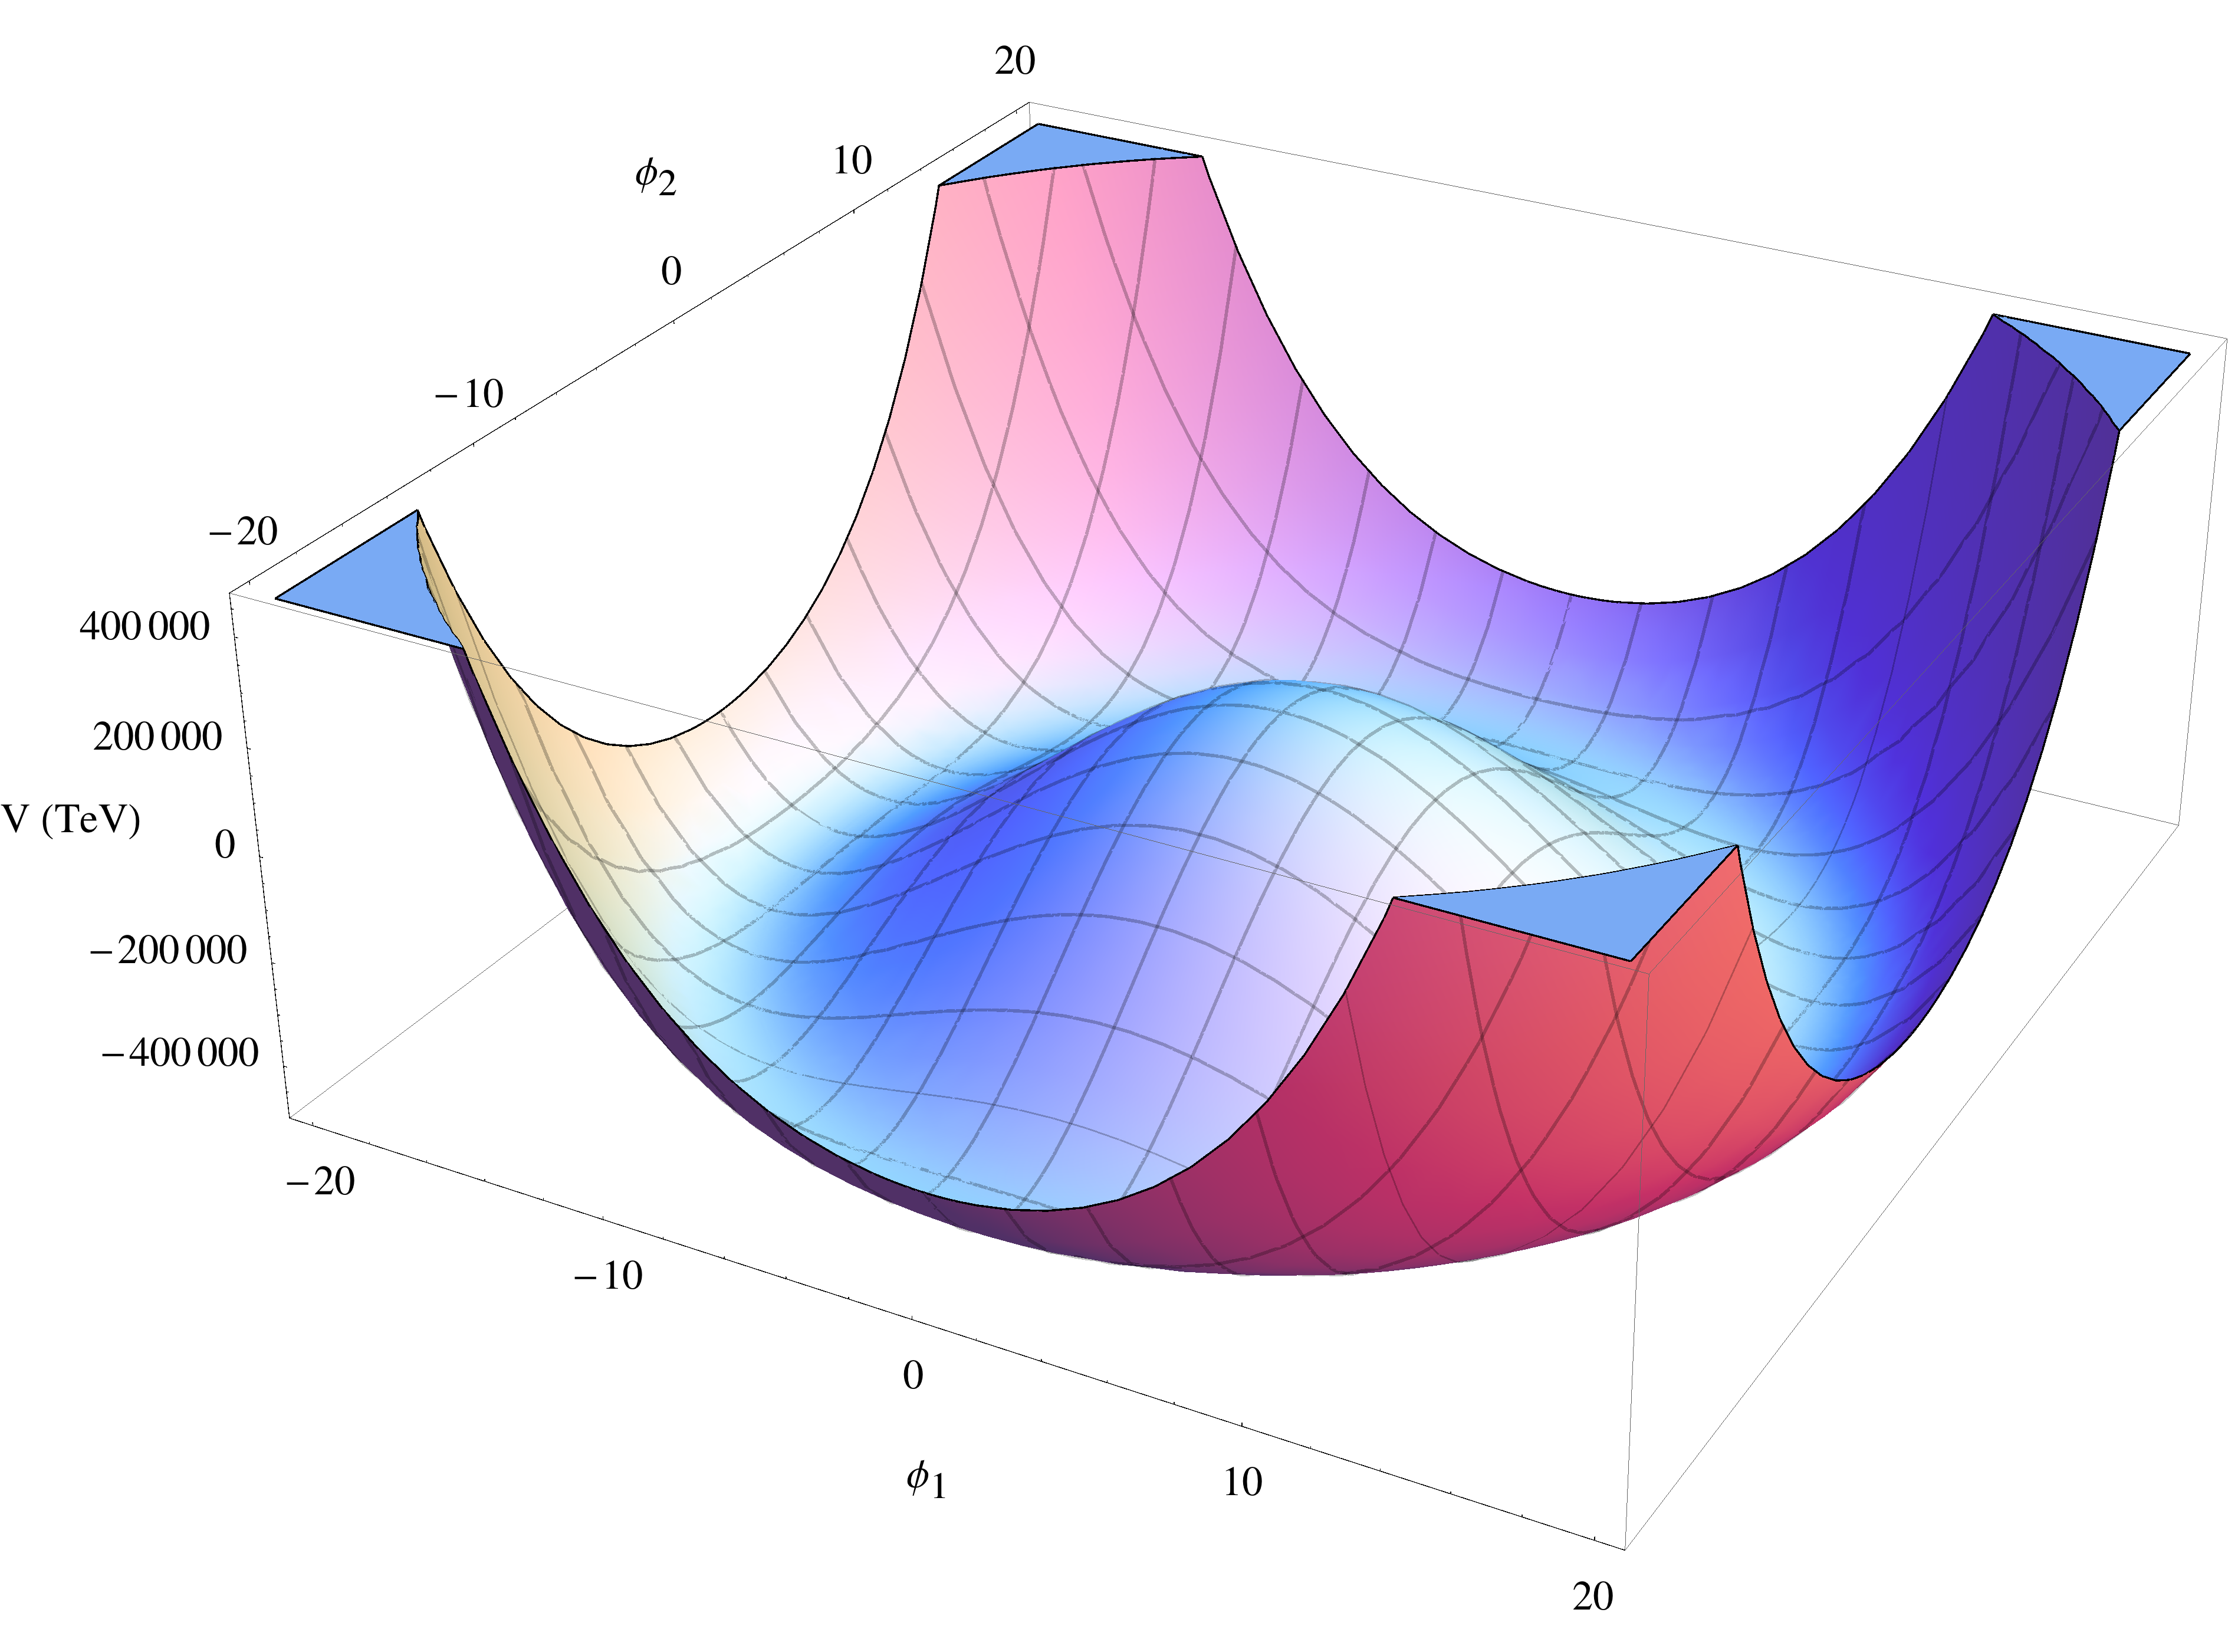
\includegraphics[width=0.6\linewidth]{Higgs_potential.png}
  \caption{Le potentiel de Higgs tracé avec les valeurs de $\mu^2$ et $\lambda$ calculées pour $m_{h} = \SI{125.3}{\GeVc}$}
\end{figure}

\subsection{Le mécanisme de Higgs}

Nous sommes intéressés par un mécanisme qui nous permet d'introduire une masse pour les médiateurs de l'interaction faible. On brise la symétrie $SU(2)_L \times U(1)_Y$ en introduisant un champ scalaire, doublet d'isospin, interagissant avec les quatre champs vectoriels $\vec{W}_\mu$ et $B_\mu$. On ajoute ainsi un terme $\mathcal{L}_2$ au Lagrangien $\mathcal{L}_\text{EWK}$ \eqref{eq:l_ewk}
\begin{align} \label{eq:l_higgs_ewk}
  \mathcal{L}_2 &= \left( \dmu \phi \right)^\star \left( \dmu \phi \right) - V(\phi)
\end{align}

On impose l'invariance locale de jauge sous une transformation de $SU(2)_L \times U(1)_Y$
\begin{align*}
  \phi \rightarrow e^{i\vec{\theta}(x) \cdot \vec{T}\,+\,i\iota(x) Y} \phi
\end{align*}

Cette invariance introduit les quatre champs vectoriels de l'interaction électrofaible. En procédant de façon identique aux sections précédentes, on obtient
\begin{align*}
  \mathcal{L}_2 &= \left| \left( i \dmu - g_1 \frac{1}{2} \vec{\tau} \cdot \vec{W}_\mu - g_2 \frac{Y}{2} B_\mu \right) \phi \right|^2 - V(\phi)
\end{align*}

On choisit comme champ scalaire un doublet d'isospin d'hypercharge $Y = 1$
\begin{align*}
 \phi &= \colvec{2}{\phi^+}{\phi^0} \quad \text{avec} \quad \begin{aligned}
    \phi^+ &= \frac{1}{\sqrt{2}} ( \phi_1 + i \phi_2 ) \\
    \phi^0 &= \frac{1}{\sqrt{2}} ( \phi_3 + i \phi_4 )
  \end{aligned}
\end{align*}

$V(\phi)$ est le potentiel de Higgs, qui admet comme minimum
\begin{align*}
  \frac{1}{2} ( \phi_1^2 + \phi_2^2 + \phi_3^2 + \phi_4^2 ) = - \frac{\mu^2}{2\lambda}
\end{align*}

Sans perte de généralité, on choisit un minimum défini par
\begin{align*}
  \phi_1 = \phi_2 = \phi_4 = 0, \quad \phi_3^2 = v^2 = - \frac{\mu^2}{2\lambda}
\end{align*}

On réexprime le champ scalaire par son expansion autour du minimum
\begin{align*}
  \phi(x) = \frac{1}{\sqrt{2}} \colvec{2}{0}{v + \eta(x) + i \frac{\vec{\tau}}{2} \cdot \vec{\xi}(x) } \simeq \frac{1}{\sqrt{2}} \exp{\left[i\frac{\vec{\tau} \cdot \vec{\xi}(x)}{2v}\right]} \colvec{2}{0}{v + \eta(x)} 
\end{align*}

En injectant $\phi$ dans le Lagrangien, on fait apparaître un terme de masse pour chacun des champs $\vec{W}_\mu$ et $B_\mu$, un terme de masse pour le champ scalaire $\eta$, mais aussi trois nouveaux champs scalaires non massifs $\vec{\xi}$. Cependant, on voit aussi apparaître des termes de la forme $\dmu \xi W^\mu$ et $\dmu \xi B^\mu$. Sous forme d'interaction, ces termes correspondent à
\begin{center} \begin{fmfgraph*}(180,30)
  \fmfleft{i1} \fmfright{o1}
  \fmf{scalar,label=$\xi$}{i1,v1}
  \fmf{boson,label=$W$}{v1,o1}
  \fmfdot{v1}
\end{fmfgraph*} \end{center}
et suggèrent que nous n'avons pas correctement identifié les particules fondamentales dans le Lagrangien. Celui ci étant invariant de jauge, nous sommes libres de choisir n'importe quelle jauge pour l'exprimer, et en particulier une jauge qui permet d'obtenir $\vec{\xi} = \vec{0}$. En remplaçant $\eta$ par $h$, on choisit comme transformation
\begin{align*}
  \phi(x) \rightarrow \frac{1}{\sqrt{2}} e^{i\vec{\theta}(x) \cdot \vec{T}\,+\,i\iota(x) Y} \colvec{2}{0}{v + h(x)}
\end{align*}

Pour conserver l'invariance par transformation de jauge locale, les champs $\vec{W}_\mu$ et $B_\mu$ se transforment maintenant de façon à faire disparaître les champs scalaires $\vec{\xi}$! Il ne reste plus que le champ scalaire $h(x)$ dans le Lagrangien: c'est le champ de Higgs.

\bigskip

Afin d'obtenir les termes de masse associés aux champs $\vec{W}_\mu$, on remplace dans le Lagrangien \eqref{eq:l_higgs_ewk} $\phi$ par sa valeur au minimum
\begin{align*}
  \phi(x) = \frac{1}{\sqrt{2}} \colvec{2}{0}{v}
\end{align*}

On obtient alors
\begin{align*}
&\left| \left( - g_1 \frac{1}{2} \vec{\tau} \cdot \vec{W}_\mu - g_2 \frac{1}{2} B_\mu \right) \phi \right|^2 \\
& \quad = \frac{1}{8} \left| \begin{pmatrix}
  - g_1 W^3_\mu - g_2 B_\mu & -g_1 \left( W^1_\mu -i W^2_\mu \right) \\
  -g_1 \left( W^1_\mu + i W^2_\mu \right) &  g_1 W^3_\mu - g_2 B_\mu
\end{pmatrix} \colvec{2}{0}{v} \right|^2 \\
& \quad = \left( \frac{1}{2} v g_1 \right)^2 W^+_\mu W^{- \mu} + \frac{1}{8} v^2 \rowvec{2}{W^3_\mu}{B_\mu} \begin{pmatrix}
   g_1^2 & - g_1 g_2 \\
   - g_1 g_2 & g_2^2
 \end{pmatrix} \colvec{2}{W^3_\mu}{B_\mu}
\end{align*}

Le premier terme est le terme de masse des bosons chargés, $W^{\pm}$. On a
\begin{align*}
  M_{W^{\pm}} &= \frac{1}{2} v g_1
\end{align*}

Le dernier terme contient les champs $W^3_\mu$ et $B_\mu$. On a vu précédemment que ces champs ne peuvent pas être interprétés comme les bosons $Z^0$ et $\gamma$, puisque $W^3$ ne couple que des particules d'hélicité gauche. Cependant, on constate que ce terme comporte des éléments non diagonaux : le mécanisme de Higgs fait apparaître naturellement un mélange entre les champs $W^3_\mu$ et $B_\mu$ pour donner naissance aux champs $Z_\mu$ et $A_\mu$.
\begin{align*}
  \frac{1}{8} v^2 \rowvec{2}{W^3_\mu}{B_\mu} \begin{pmatrix}
   g_1^2 & - g_1 g_2 \\
   - g_1 g_2 & g_2^2
 \end{pmatrix} \colvec{2}{W^3_\mu}{B_\mu} &= \frac{1}{8} v^2 \left( g_1W^3_\mu - g_2 B_\mu \right)^2 + 0 \left( g_2 W^3_\mu + g_1B_\mu \right) \\
 &= \frac{1}{8} v^2 \left(g_1^2 + g_2^2\right) Z_\mu^2 + 0 A_\mu^2
\end{align*}
avec
\begin{align*}
  Z_\mu &= \frac{g_1W^3_\mu - g_2 B_\mu}{\sqrt{g_1^2 + g_2^2}} & & & A_\mu &= \frac{g_2W^3_\mu + g_1 B_\mu}{\sqrt{g_1^2 + g_2^2}} \\  
\end{align*}

Le terme de masse d'un boson vecteur neutre étant de la forme $\frac{1}{2} M_V^2 V_\mu^2$, on identifie
\begin{align*}
  M_Z &= \frac{1}{2} v \sqrt{g_1^2 + g_2^2} & & & M_A &= 0
\end{align*}

L'introduction d'un nouveau champ scalaire se couplant  à $\vec{W_\mu}$ et à $B_\mu$ permet, grâce au mécanisme de Higgs, de générer une masse pour les médiateurs de l'interaction faible, tout en gardant le photon non massif. On peut réexprimer le mélange entre $W^3_\mu$ et $B_\mu$ en introduisant l'angle de mélange $\theta_W$ (angle de Weinberg), et en posant
\begin{align*}
  \frac{g_2}{g_1} &= \tan \theta_W
\end{align*}

On obtient alors
\begin{align} \label{eq:ewk_mixing}
  \colvec{2}{A_\mu}{Z_\mu} &= \begin{pmatrix}
    \cos \theta_W & \sin \theta_W \\
    - \sin \theta_W & \cos \theta_W
  \end{pmatrix} \colvec{2}{B_\mu}{W^3_\mu}
\end{align}
et
\begin{align*}
  \frac{M_W}{M_Z} &= \cos \theta_W
\end{align*}

Connaissant maintenant l'existence d'un mélange entre les bosons $W^3_\mu$ et $B_\mu$, on peut injecter \eqref{eq:ewk_mixing} dans \eqref{eq:l_ewk}. En ne considérant que la partie neutre du Lagrangien, on obtient
\begin{align*}
  \mathcal{L}_{\text{neutre}} &= \bar{\chi}_L \gmuc \left( -g_1 T^3 W^3_\mu -g_2 \frac{Y}{2} B_\mu \right) \chi_L + \Psib_R \gmuc \left(-g_2 \frac{Y}{2} B_\mu \right) \Psi_R \\
  &\begin{aligned} =\ &\bar{\chi}_L \gmuc \left( \left\{ -g_1 T^3 \sin\theta_W -g_2 \frac{Y}{2} \cos\theta_W \right\} A_\mu \right. \\
                     +&\hphantom{\bar{\chi}_L \gmuc \left(\vphantom{\frac{Y}{2}}\right.} \left. \left\{ -g_1 T^3 \cos\theta_W + g_2 \frac{Y}{2} \sin\theta_W \right\} Z_\mu \right) \chi_L\\
                     +&\Psib_R \gmuc \left( \left\{-g_2 \frac{Y}{2} \cos\theta_W\right\}A_\mu + \left\{ g_2 \frac{Y}{2} \sin\theta_W \right\} Z_\mu \right) \Psi_R
                     \end{aligned}
\end{align*}

On sait que le couplage au photon, obtenu grâce au Lagrangien QED \eqref{eq:l_qed}, est de la forme $e Q A_\mu$. En utilisant la relation \eqref{eq:q_t_y}, on trouve que les couplages $g_1$ et $g_2$ doivent satisfaire la relation suivante
\begin{align*}
  g_1 \sin\theta_W = g_2 \cos\theta_W = e
\end{align*}

Les couplages de l'interaction électrofaible ne sont pas indépendants, et sont reliés à la charge électrique.

\subsection{Champ de Higgs et masses des fermions}

On a vu précédemment que le champ scalaire introduit présentait un minimum de potentiel obtenu pour une valeur $\phi \neq 0$. On réexprime donc $\phi$ par une expansion autour de son minimum $v$
\begin{align*}
  \phi(x) = \frac{1}{\sqrt{2}} \colvec{2}{0}{v + h(x)}
\end{align*}

En injectant $\phi$ dans le potentiel $V(\phi)$, on obtient
\begin{align*}
  V(\phi) &= \frac{1}{4} v^2\mu^2 - \mu^2h^2 - \frac{\mu^2}{v} h^3 + \frac{1}{4} \lambda h^4
\end{align*}

Le champ de Higgs est donc massif, et on a $m_h = \sqrt{-\mu^2} = \sqrt{2v^2 \lambda}$, nouveau paramètre libre de la théorie. Les deux derniers termes représentent l'interaction du champ de Higgs avec lui même (à trois et quatre vertex). On dit qu'il est auto-couplant.

\bigskip

Dans le Lagrangien électrofaible \eqref{eq:l_ewk}, le terme de masse des fermions n'a pas pu être inclus puisqu'il brisait l'invariance locale de jauge. En effet, si on considère le terme $m\Psib\Psi$, on a
\begin{align*}
  m \Psib \Psi &= m \Psib \left[ \frac{1}{2} \left(1 - \gfivec\right) + \frac{1}{2} \left(1 + \gfivec\right) \right] \Psi \\
  &= m \left[ \Psib_R \Psi_L + \Psib_L \Psi_R \right]
\end{align*}

Ce terme dépend donc à la fois des composantes de chiralité gauche et droite du champ. Or, ces quantités ne se transforment pas de la même façon sous une transformation $SU(2)_L \times U(1)_Y$ : l'invariance est brisée.

Il s'avère que le même doublet de Higgs peut aussi générer la masse des fermions du Modèle Standard. On procède de façon analogue à la section précédent, et on introduit dans le Lagrangien un terme invariant sous $SU(2)_L \times U(1)_Y$ :
\begin{align*}
  \mathcal{L}_3 &= -G_f \left[ \rowvec{2}{\bar{\nu}}{\bar{f}}_L \phi f_R + \bar{f}_R \phi^\dagger \colvec{2}{\nu}{f}_L \right] \qquad f = e, \mu, \tau
\end{align*}

On substitue $\phi$ par son expansion autour du minimum, et on obtient
\begin{align*}
  \mathcal{L}_3 &= -\frac{G_f}{\sqrt{2}} v (\bar{f}_L f_R + \bar{f}_R f_L) -\frac{G_f}{\sqrt{2}} v (\bar{f}_L f_R + \bar{f}_R f_L)h
\end{align*}

Les leptons acquièrent donc une masse $m_f = \frac{G_f v}{\sqrt{2}}$. Le dernier terme représente quant à lui l'interaction des leptons avec le champ de Higgs, avec un couplage proportionnel à la masse. On introduit donc trois nouveaux paramètres libres dans la théorie, un pour chaque fermion : ce sont les couplages de Yukawa des leptons au champ de Higgs.

Intéressons nous maintenant aux quarks. Leur masse est générée de façon identique, à une différence près : il faut un moyen de générer une masse pour les quarks de type \emph{up} qui, contrairement aux neutrinos, ont une masse. On introduit un nouveau doublet de Higgs $\phi_C$, qui se transforme de façon identique à $\phi$, et qui se couple aux quarks de type \emph{up}
\begin{align*}
  \phi_C &= -i \tau_2 \phi^\star = \colvec{2}{- \bar{\phi}^0}{\phi^-} \xrightarrow[\text{brisure de symétrie}]{} \frac{1}{\sqrt{2}} \colvec{2}{v + h}{0}
\end{align*}

Le nouveau terme à insérer dans le Lagrangien est
\begin{align*}
  \mathcal{L}_4 &= -G_d^{ij} \rowvec{2}{\bar{u}_i}{\bar{d}_i^\prime} \colvec{2}{\phi^+}{\phi^0} d_{jR} - G_u^{ij} \rowvec{2}{\bar{u}_i}{\bar{d}_i^\prime} \colvec{2}{- \bar{\phi}^0}{\phi^-} u_{jR} + \text{conjugué hermitien}
\end{align*}

On substitue $\phi$ par son expansion autour du minimum, et on obtient
\begin{align*}
  \mathcal{L}_4 &= - m_d^i \bar{d}_i d_i \left( 1 + \frac{h}{v} \right) - m_u^i \bar{u}_i u_i \left( 1 + \frac{h}{v} \right)
\end{align*}

Comme pour le cas des fermions, on introduit six nouveaux paramètres libres dans la théorie, un pour chaque quark.

\bigskip

\begin{figure}
  \subcaptionbox{\label{fig:higgs_mgg}}[.45\linewidth]{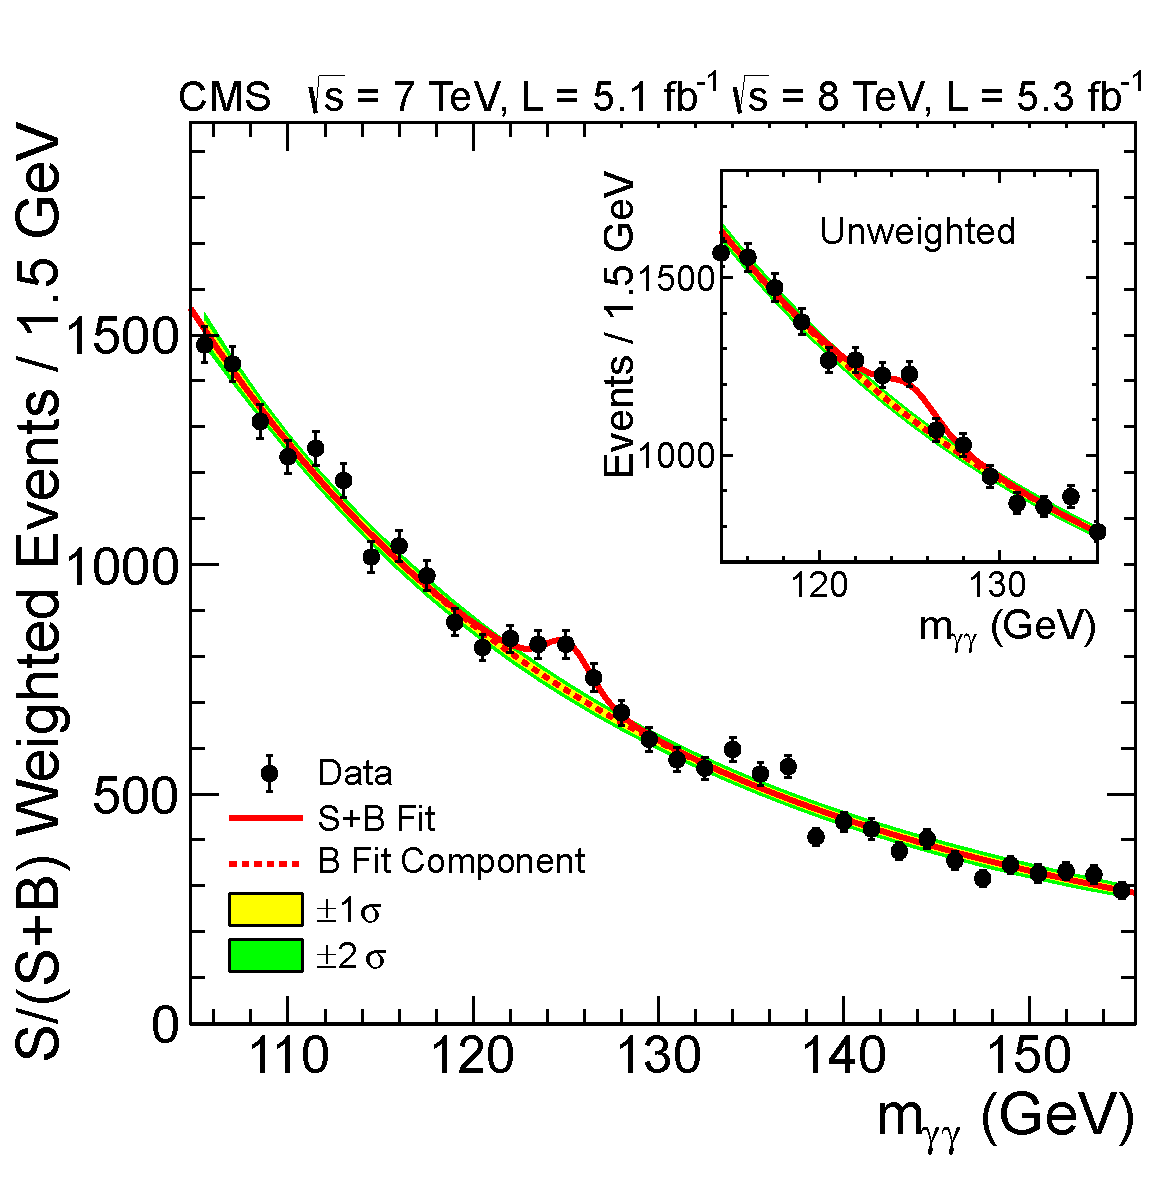
\includegraphics[width=0.45\textwidth]{higgs_mgg.pdf}}\hfill
  \subcaptionbox{\label{fig:higgs_pvalue}}[.45\linewidth]{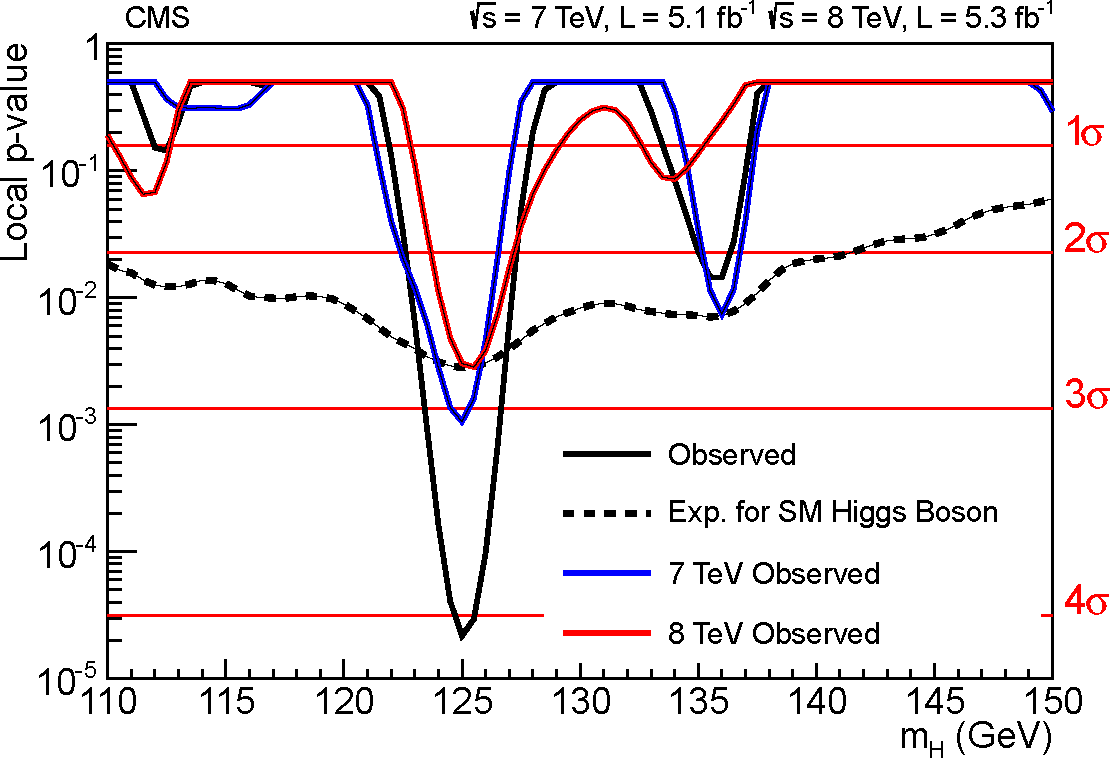
\includegraphics[width=0.45\textwidth]{higgs_pvalue.pdf}}
  \caption{A gauche, spectre de masse invariante $H \rightarrow m_{\gamma\gamma}$. A droite, la \emph{p-value} associée à cette mesure, qui correspondant à la probabilité que la mesure soit compatible avec une absence de signal. On voit clairement la présence d'une nouvelle particule aux alentours de \SI{125}{\GeV}.}
\end{figure}

Au travers de la brisure de symétrie et du mécanisme de Higgs, on a pu voir comment les bosons de jauges $W$ et $Z$, les leptons et les quarks acquièrent une masse.
\begin{itemize}
  \item Les masses des bosons de jauge faible s'exprime à l'aide de $\mu^2$ et $\lambda$, les paramètres du potentiel de Higgs.
  \item Les masses des fermions deviennent des paramètres libres de la théorie.
\end{itemize}

Le mécanisme de Higgs prévoit donc l'existence d'un nouveau champ scalaire, le champ de Higgs. Le boson associé a une masse $m_h = \sqrt{2v^2\lambda}$. Plus de 30 ans après sa prédiction, le CERN a officiellement annoncé le 4 juillet 2012 la découverte d'une nouvelle particule compatible avec le boson de Higgs \citep{higgs_cms,higgs_atlas}. Cette particule a été observée dans plusieurs canaux de désintégration, dont $H \rightarrow \gamma\gamma$ et $H \rightarrow ZZ$. On peut voir figure \ref{fig:higgs_mgg} le spectre de masse invariante $m_{\gamma\gamma}$ pour l'expérience CMS, où on voit clairement une déviation par rapport à la prédiction théorique, et figure \ref{fig:higgs_pvalue} la \emph{p-value} associée à la découverte. La \emph{p-value} représente la probabilité que la mesure soit compatible avec une absence de signal. On remarque la très nette déviation autour de \SI{125}{\GeV}.

% Des signes sont aussi présent dans la désintégration $\tau\tau$, ce qui serait la preuve qu'il est en effet correct d'étendre le mécanisme de Higgs pour générer la masse des fermions.
Selon les derniers résultats, ce boson a une masse de $m_h = \SI{125.9 \pm 0.4}{\GeV}$ \citep{pdg}. De nombreuses recherches sont encore en cours afin de déterminer si ce boson est bien celui prédit par le Modèle Standard, mais les premiers résultats laissent à penser que c'est le cas.

% \subsection{Renormalisation} \label{sec:renormalisation}

% Lorsque l'on ajoute des boucles aux diagrammes d'un processus à l'arbre, le calcul de l'élément de matrice de transition diverge. Par exemple, lors du passage du diagramme \ref{fig:ee_annihilation} au diagramme \ref{fig:ee_annihilation_high_order}, il est nécessaire d'intégrer sur toutes les impulsions possibles, puisque la particule qui forme la boucle est virtuelle. Ceci entraîne l'apparition de terme de la forme $\int k dk$, avec $k \rightarrow \infty$. termes qui divergent.

% \begin{figure}[t] \centering
%   \subcaptionbox{\label{fig:ee_annihilation}}[.4\linewidth]{
%   \begin{fmfgraph*}(180,100)
%     \fmfpen{0.5}
%     \fmfleft{i1,i2}
%     \fmfright{o1,o2}
%     \fmf{fermion}{i1,v1,i2}
%     \fmf{fermion}{o1,v2,o2}
%     \fmfdot{v1} \fmfdot{v2}
%     \fmf{photon,label=$\gamma$}{v1,v2}
%     \fmflabel{$e^-$}{i1} \fmflabel{$e^+$}{i2} 
%     \fmflabel{$e^+$}{o1} \fmflabel{$e^-$}{o2} 
%   \end{fmfgraph*}}\qquad%
% %   \subcaptionbox{\label{fig:ee_annihilation_high_order}}[.4\linewidth]{
% %   \begin{fmfgraph*}(180,100)
% %     \fmfpen{0.5}
% %     \fmfleft{i1,i2}
% %     \fmfright{o1,o2}
% %     \fmf{fermion}{i1,g1,v1,g2,i2}
% %     \fmf{fermion,tension=0.5}{o1,v2,o2}
% %     \fmfdot{v1} \fmfdot{v2}
% %     \fmf{photon,label=$\gamma$}{v1,v2}
% %     \fmf{photon,label=$\gamma$,tension=0,left=0.7}{g1,g2}
% %     \fmflabel{$e^-$}{i1} \fmflabel{$e^+$}{i2} 
% %     \fmflabel{$e^+$}{o1} \fmflabel{$e^-$}{o2} 
% %   \end{fmfgraph*}}
%   \subcaptionbox{\label{fig:ee_annihilation_high_order}}[.4\linewidth]{
%   \begin{fmfgraph*}(180,100)
%     \fmfpen{0.5}
%     \fmfleft{i1,i2}
%     \fmfright{o1,o2}
%     \fmf{fermion}{i1,v1,i2}
%     \fmf{fermion}{o1,v2,o2}
%     \fmfdot{v1} \fmfdot{v2}
%     \fmf{photon,label=$\gamma$,tension=2}{v1,g1}
%     \fmf{photon,label=$\gamma$,tension=2}{g2,v2}
%     \fmf{fermion,left=1,label=$e^-$}{g1,g2}
%     \fmf{fermion,left=1,label=$e^+$}{g2,g1}
%     \fmflabel{$e^-$}{i1} \fmflabel{$e^+$}{i2} 
%     \fmflabel{$e^+$}{o1} \fmflabel{$e^-$}{o2} 
%   \end{fmfgraph*}}
%   \caption{Diagrammes de Feynman $e^+e^- \rightarrow e^+e^-$ d'ordre 1 (\protect\subref{fig:ee_annihilation}) et d'ordre 2 (\protect\subref{fig:ee_annihilation_high_order}).}
%   \label{fig:ee_annihilation_total}
% \end{figure}

% Néanmoins, il est possible de supprimer ces divergences en introduisant un \emph{cut-off} dans la théorie, c'est-à-dire une énergie arbitraire jusqu'où le modèle est valide. Ce nouveau paramètre est ensuite absorbé dans une redéfinition de la constante de couplage du processus, qui par conséquence n'est plus constante mais dépend de l'énergie du processus : c'est la renormalisation.

% \bigskip

% Pour l'interaction électromagnétique, la constante de couplage $\alpha_0$ devient, après renormalisation
% \begin{align*}
%   \alpha\left(Q^2\right) &= \frac{\alpha(\mu^2)}{1 - \frac{\alpha(\mu^2)}{2\pi} \ln\left( \frac{Q^2}{\mu^2} \right) }
% \end{align*}
% où $Q^2$ est l'énergie à laquelle évaluer la constante de couplage, et $\mu^2$ la valeur de l'échelle de renormalisation.

% Dans le cas de l'interaction forte, la constante de couplage $\alpha_s$ devient
% \begin{align*}
%   \alpha_s\left(Q²\right) &= \frac{\alpha_s(\mu^2)}{1 + \frac{\alpha_s(\mu^2)}{12\pi} \left(33 - 2n_f\right) \ln\left( \frac{Q^2}{\mu^2} \right) }
% \end{align*}
% où $n_f$ est le nombre de saveurs (6 quarks). Une chose importante à noter est que la constante de couplage de l'interaction forte \emph{diminue} avec l'énergie, and devient faible pour des faibles distances d'interaction : c'est la liberté asymptotique. A l'inverse, plus la distance d'interaction augmente, plus l'interaction est importe : à partir d'une certaine distance, l'énergie disponible est suffisante pour créer une paire $q\bar{q}$. Il n'est ainsi pas possible d'observer un quark seul, c'est le confinement.

% On définit une nouvelle échelle, $\Lambda^2$, définit comme la valeur à laquelle la constante de couplage devient trop importante pour que le calcul perturbatif puisse être utilisé. On a
% \begin{align*}
%   \Lambda^2 &= \mu^2 \exp\left( \frac{-12\pi}{(33 - 2n_f) \alpha_s\left(\mu^2\right)} \right) \\
%   \alpha_s\left(Q^2\right) &= \frac{12 \pi}{\left(33 - 2n_f\right) \ln\left( \frac{Q^2}{\Lambda^2} \right)}
% \end{align*}

% On peut voir $\Lambda$ comme la frontière entre le monde des quarks libres, décrit correctement par des calculs perturbatifs, et le monde des quarks liés. Afin de décrire ces états, les calculs perturbatifs ne sont pas correct, la constante de couplage étant grande devant l'unité. On peut utiliser des techniques de simulation telle que la QCD sur réseau \citep{PhysRevD.10.2445}.

\section{Faiblesses du Modèle Standard} \label{sec:sm_weakness}

Depuis son développement dans les années 1960, le Modèle Standard est un succès expérimental. Il a en effet prédit l'existence des bosons $W^{\pm}$, $Z$, des quarks $b$ et $t$ avant leur découverte. Si l'on exclu la récente découverte d'une particule compatible avec le boson de Higgs en 2012, la dernière découverte est celle du quark $t$ en 1995 au Tevatron, l'accélérateur de particule du Fermilab, aux États-Unis. On présente figure \ref{fig:ewk_fit} les derniers résultats de l'ajustement des paramètres de la théorie électrofaible. En effet, le Modèle Standard permet de relier quasiment tous les paramètres par des relations. L'ajustement permet donc de comparer directement les prédictions du Modèle Standard avec les mesures expérimentales. Les différences entre les valeurs expérimentales et les valeurs ajustées sont toutes inférieures à 3 $\sigma$, démonstration du succès du Modèle Standard.

Malgré ce succès qui dure depuis plus de 50 ans, un certain nombre d'interrogations et de problèmes demeurent. En effet, un certain nombre d'éléments laissent à penser que le Modèle Standard n'est qu'un modèle effectif à basse énergie d'une théorie plus fondamentale.

\begin{figure} \centering
  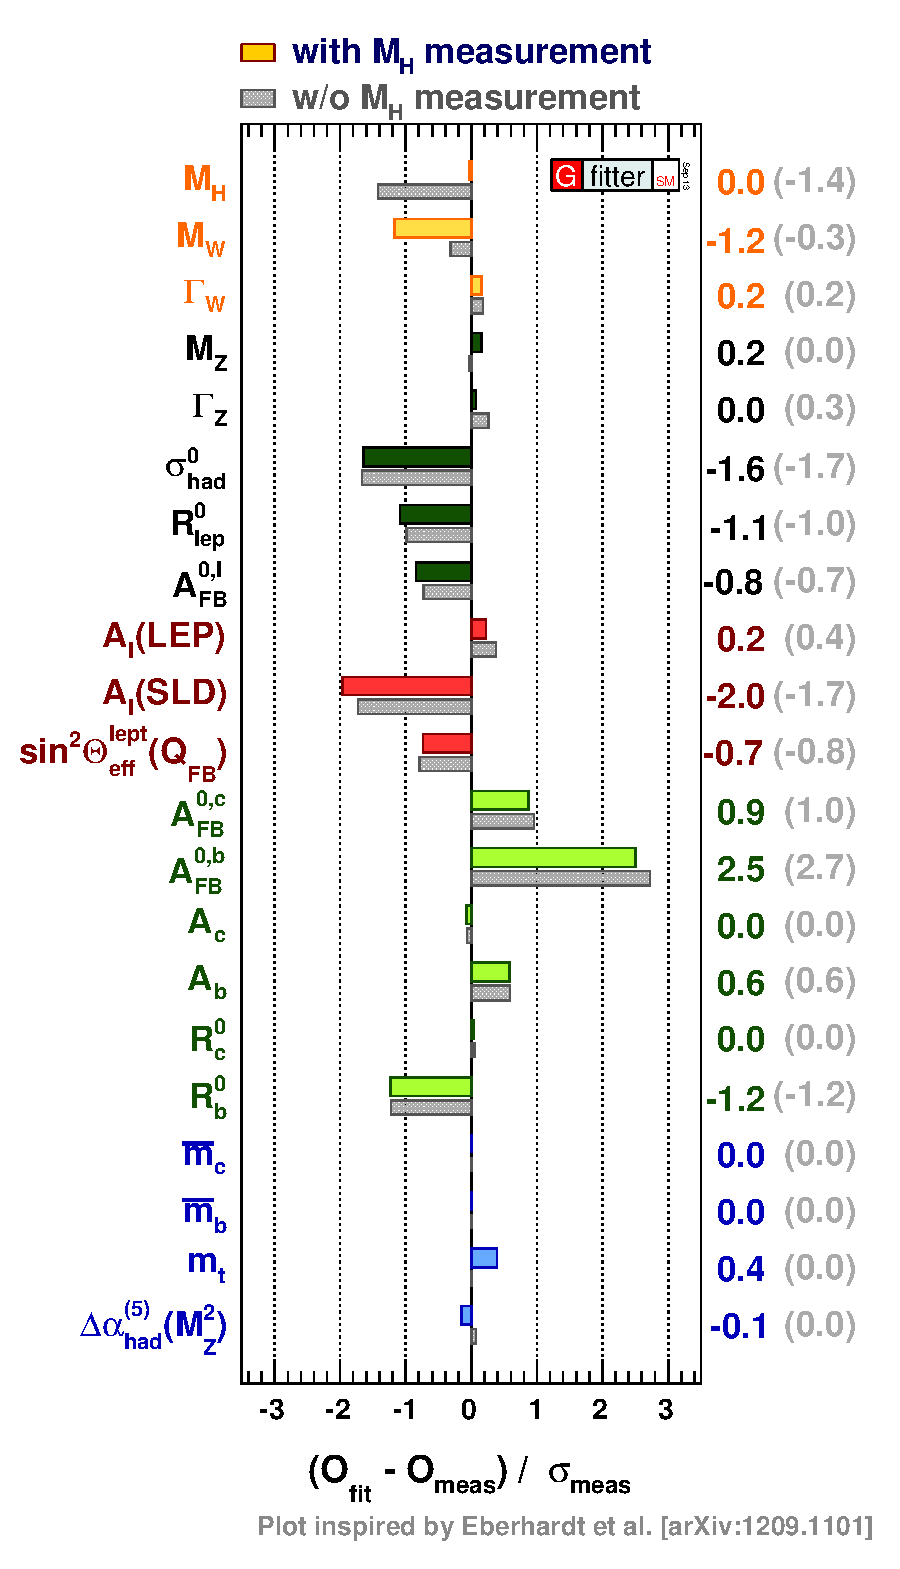
\includegraphics[height=0.9\textheight]{PullPlotTwoBarsCol_logo.eps}
  \caption{Comparaison entre les valeurs expérimentales et les valeurs ajustées des principales observables de la théorie électrofaible du Modèle Standard, pour deux cas de figures : en couleur, l'ajustement inclut la découverte du probable boson de Higgs ; en gris, ce résultat n'est pas utilisé. Les valeurs à droite correspondent au \emph{pull}, c'est-à-dire à la différence entre la valeur expérimentale et la valeur ajustée, exprimée en sigma, où 1$\sigma$ correspond à un intervalle de confiance de \SI{68.2}{\%}. Les faibles écarts observés ($<$ à 3 $\sigma$) sont une démonstration du succès du Modèle Standard. Résultats issus de \citep{ewk_fit}.}
  \label{fig:ewk_fit}
\end{figure}

\begin{description}
  \item[Nombre de paramètres libres] Tel que construit, le Modèle Standard comporte 19 paramètres libres : les 6 masses des quarks, les 3 masses des leptons, l'angle de mélange électrofaible, les 4 paramètres de la matrice CKM, les 3 constantes de couplage, et les deux paramètres du potentiel de Higgs. L'un des objectifs majeur de la Physique étant de décrire de façon la plus simple possible les phénomènes, tout laisse à penser qu'une théorie comportant moins de paramètres libres engloberait le Modèle Standard.
  \item[Nombre de générations] Les contraintes sur le nombre de générations de leptons proviennent des mesure de la largeur du $Z$, et conduisent à une prédiction de 3 générations. Néanmoins, une quatrième génération plus massive que la masse du $Z$ ou non couplée à l'interaction faible n'est pas exclue ; le Modèle Standard ne prédit pas le nombre de générations de fermions.
  \item[L'ajustement fin] Les diagrammes de Feynman qui contribuent au calcul de la masse du boson de Higgs incluent des boucles, qui conduisent à des divergences. Le Modèle Standard étant une théorie renormalisable, ces divergences peuvent être absorbées dans la masse du boson, conduisant à une masse effective ($m_h$) différente de la masse nue ($m_{h, 0}$) \citep{higgs_mass} :
  \begin{align*}
    m_h^2 &= m_{h, 0}^2 - \frac{3 \Lambda^2}{8 \pi^2 v^2} \left(m_h² + 2m_W^2 + m_Z^2 - 4m_t\right)
  \end{align*}
  où $\Lambda$ est le \emph{cut-off} (la limite haute de l'intégrale). Si on considère le Modèle Standard valide jusqu'à l'échelle de la grande unification ($\Lambda = \SI{\tilde e16}{\GeV}$), et un boson de Higgs avec $m_h = \SI{125}{\GeV}$, il est nécessaire de procéder à un ajustement jusqu'à la vingtième décimale entre la masse nue du boson et les corrections radiatives. Cet ajustement fin suggère l'existence d'autres processus qui viendraient naturellement annuler ces corrections radiatives.
  \item[Quantification de la charge électrique] On sait par l'expérience que la charge électrique est quantifiée, et doit être un multiple de $e = \SI{1.602176565(35)}{\coulomb}$ ($1$ pour les leptons, $\sfrac{1}{3}$ pour les quarks). L'opérateur de charge $Q$ est introduit afin de reproduire cette quantification, mais aucune justification théorique n'est donnée dans le cadre du le Modèle Standard.
\begin{figure} \centering
  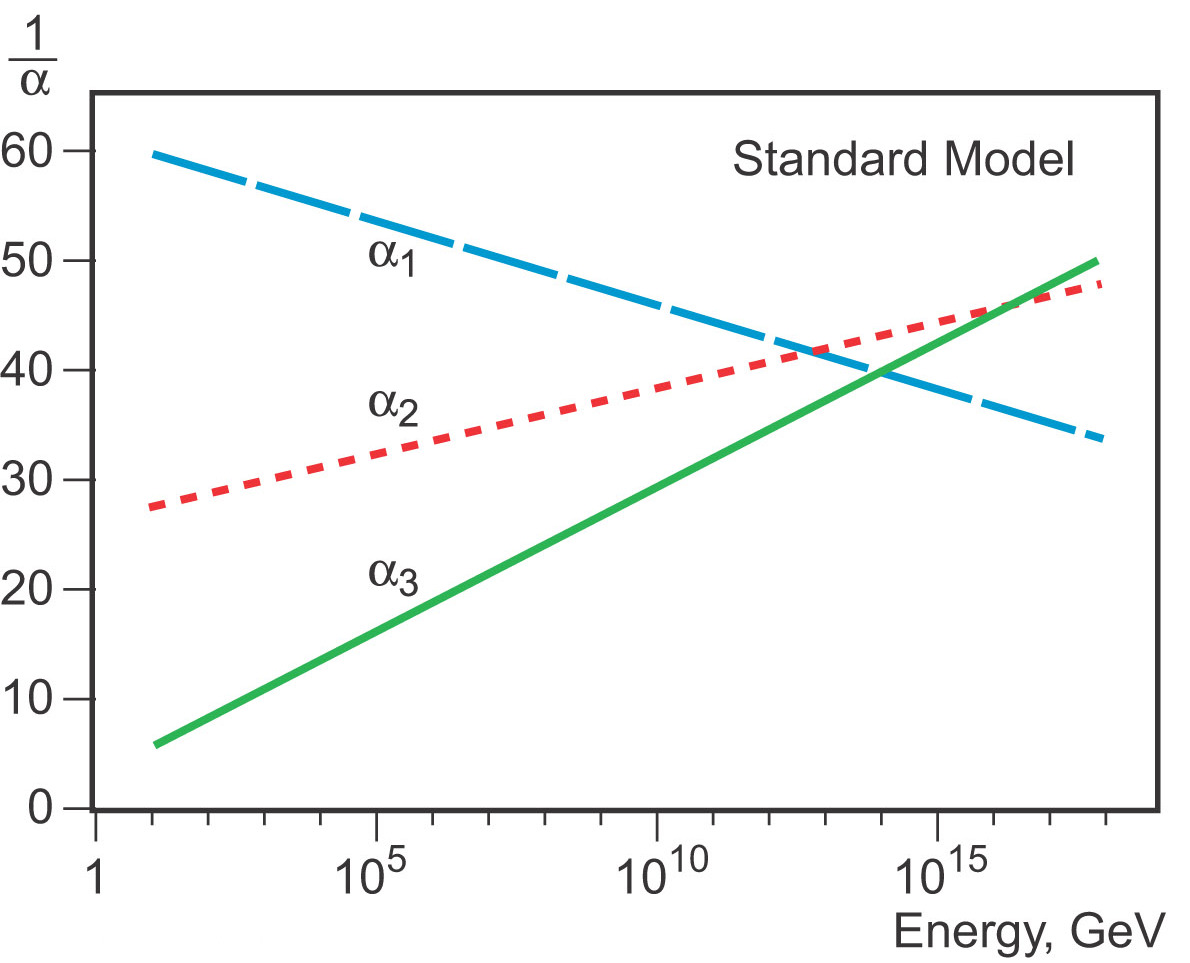
\includegraphics[width=0.5\linewidth]{running_coupling.jpg}
  \caption{L'évolution des constantes de couplages du Modèle Standard en fonction de l'énergie. On remarque qu'à une certaine énergie, les constantes de couplages semblent être identique : un signe d'une possible unification des interactions ?}
  \label{fig:unification}
\end{figure}
  \item[Grande unification] On peut voir figure \ref{fig:unification} l'évolution des constantes de couplage en fonction de l'énergie. Ces constantes semblent tendre à s'unifier à une certaine énergie, ce qui pourrait indiquer une possible unification entre les trois interactions. De nombreux modèles au-delà du Modèle Standard modifient les couplages de façon à ce que les trois interactions se croisent en un unique point.
  \item[Neutrinos] Le Modèle Standard que l'on vient de bâtir prévoit des neutrinos sans masse. La découverte de l'oscillation des neutrinos (\tilde 1970 avec la découverte de l'oscillation des neutrinos solaires) impose néanmoins aux neutrinos d'être massifs. De façon analogue aux quarks, il est possible d'inclure dans le Modèle Standard un terme supplémentaire afin de permettre aux neutrinos d'acquérir une masse grâce au mécanisme de Higgs. Il reste cependant à expliquer pourquoi il existe une telle différence de masse entre les leptons et les neutrinos (\SI{511}{\keV} contre \SI{\tilde 1}{\eV}). La solution pourrait venir du mécanisme de \emph{see-saw}. En effet, l'existence de neutrinos massifs impose l'existence de neutrinos de chiralité droite. Si on postule que ces neutrinos droits sont des particules de Majorana\footnote{Une particule de Majorana est une particule étant sa propre anti-particule.}, il est possible d'ajouter au Lagrangien, en plus du terme de masse de Higgs, un nouveau terme de masse, invariant sous une transformation $SU(2)_L \times U(1)_Y$, de la forme :
\begin{align*}
  \mathcal{L} &= \frac{-M}{2} \left[ \left(\nu_R^C\right)^\dagger \nu_R + \nu_R^\dagger \nu_R^C \right] \\
              &= \frac{-M}{2} \left[ \nu_R^\dagger \nu_R + \nu_R \nu_R^\dagger \right]
\end{align*}
où l'exposant $C$ correspondant à la conjugaison de charge. En combinant ce terme avec celui obtenu par le mécanisme de Higgs, on trouve
\begin{align*}
  \mathcal{L} &= \rowvec{2}{\nu_L^\dagger}{\nu_R^\dagger} \begin{pmatrix}
    0 & m_D\\
    m_D & M
  \end{pmatrix} \colvec{2}{\nu_L}{\nu_R}
\end{align*}
où $m_D$ est la masse obtenue grâce au mécanisme de Higgs, et $M$ grâce au terme de Majorana. Afin d'obtenir les états propres de masse, on diagonalise la matrice. Les valeurs propres sont
\begin{align*}
  m_1 &\simeq \frac{m_D^2}{M} &&& m_2 &\simeq M
\end{align*}
  
  Si on choisi comme valeur pour $m_D$ une valeur proche de la masse des fermions, et une valeur très grande pour $M$, on voit que l'on génère deux masses : une très faible, $m_1$, qui serait la masse des neutrinos gauches, et une très grande, $m_2$, qui serait la masse d'un hypothétique neutrino droit.
  
% Les neutrinos étant massif, il existe forcément des neutrinos de chiralité droite. N'ayant jamais été observés, ces neutrinos semblent insensible aux trois interactions fondamentales du Modèle Standard : il ne porte ainsi aucune charge électrique, de couleur ou faible. On peut donc considérer le neutrino droit comme une particule de Majorama, c'est-à-dire une particule étant sa propre anti-particule. Dans ce cas, il est possible d'inclure dans le Lagrangien un terme de masse invariant sous transformation de jauge locale, de la forme

\medskip
  
L'oscillation des neutrinos peut elle être expliquée de manière analogue au mélange entre les quarks. On introduit une nouvelle matrice de mélange entre les neutrinos états propres de masse et les neutrinos états propre de l'interaction faible : la matrice PMNS \citep{neutrino_mixing_1,neutrino_mixing_2}. Cette matrice est paramétrisée par trois angles de mélange et une phase. Les dernières valeurs expérimentales \citep{pdg} sont
    \begin{align*}
      \theta_{12} \simeq  \SI{34}{\degree}, \theta_{23} \simeq \SI{45}{\degree}, \theta_{13} \simeq \SI{9.1}{\degree} 
    \end{align*}
    la phase $\delta CP$ n'ayant pas encore été mesurée.
  
%   Il reste cependant à expliquer pourquoi la masse des neutrinos est si faible comparée à celle des autres leptons. En effet, les limites expérimentales pose une limite supérieure sur la masse des neutrinos \citep{pdg} de $\SI{2}{\eV}$ pour $\nu_e$, $\SI{0.19}{\MeV}$ pour $\nu_\mu$ et $\SI{18.2}{\MeV}$ pour $\nu_\tau$.
  
  \item[Gravitation] Le Modèle Standard unit sous un même formalisme mathématique les interactions électromagnétiques, faibles et fortes. La gravitation est elle décrite par la relativité générale. A l'échelle de grande unification, l'interaction gravitionnelle devient du même ordre de grandeur que les autres interactions et ne peut plus être négligée : une nouvelle théorie est alors nécessaire tenant compte de la gravité.
  
  De nombreuses tentatives ont eu lieu pour quantifier la gravitation. Elles se heurtent toutes au même problème : une fois intégrée à la théorie, celle-ci n'est plus renormalisable et conduit à des probabilités infinies. Néanmoins, les recherches continuent, et la théorie la plus prometteuse est actuellement la théorie des supercordes, qui permet d'unifier sous un même formalisme les quatre interactions fondamentales, en considérant les particules fondamentales non pas comme des particules, mais comme des cordes vibrantes.
\end{description}

% \begin{figure} \centering
%   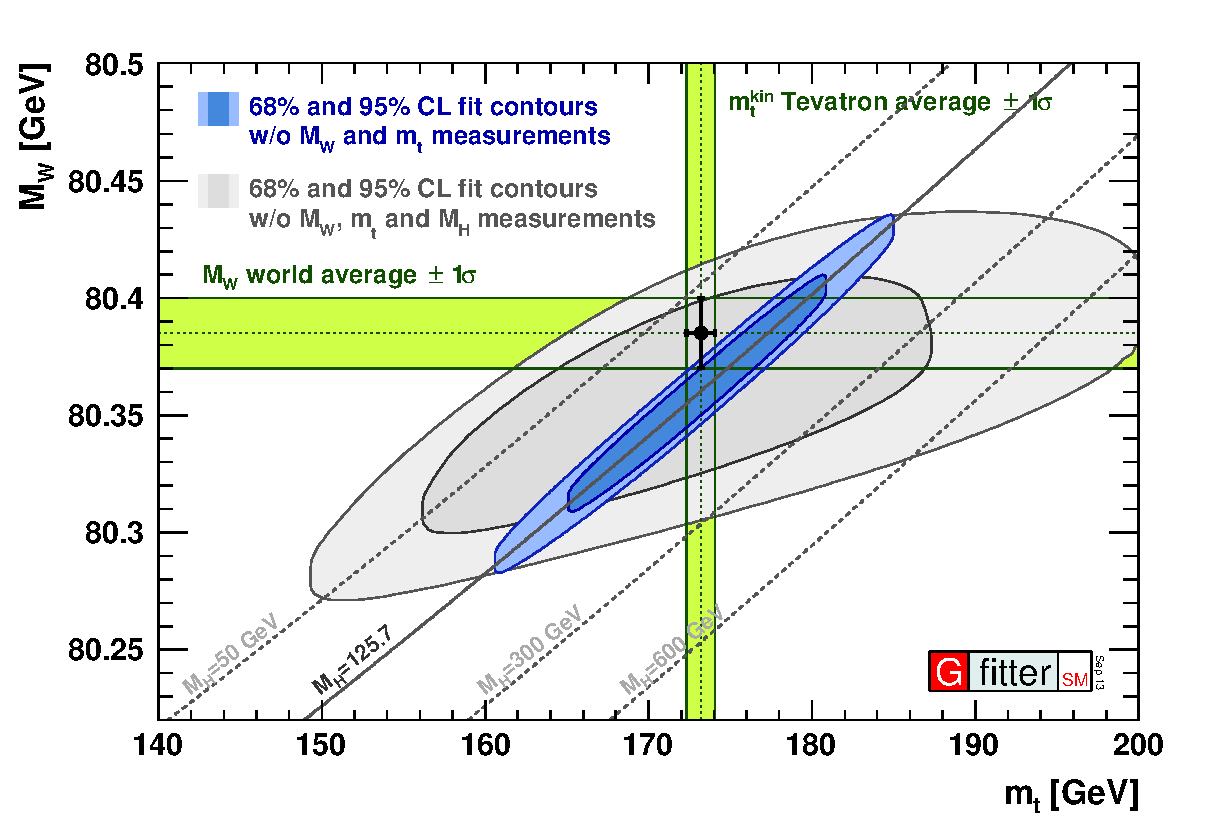
\includegraphics[width=0.55\linewidth]{W_vs_top_logo.eps}
%   \caption{Contour du fit des paramètres électrofaible du Modèle Standard en fonction de $m_t$ et $m_W$. Les valeurs expérimentales de $m_t$ et $m_W$ sont en jaune. Le contour gris n'inclue pas la valeur de $m_h = \SI{125.7}{\GeV}$ dans le fit, à la différence du contour bleue. Les prédictions théoriques sont en accord avec l'expérience.}
%   \label{fig:ewk_w_vs_top}
% \end{figure}

% \begin{figure} \centering
%   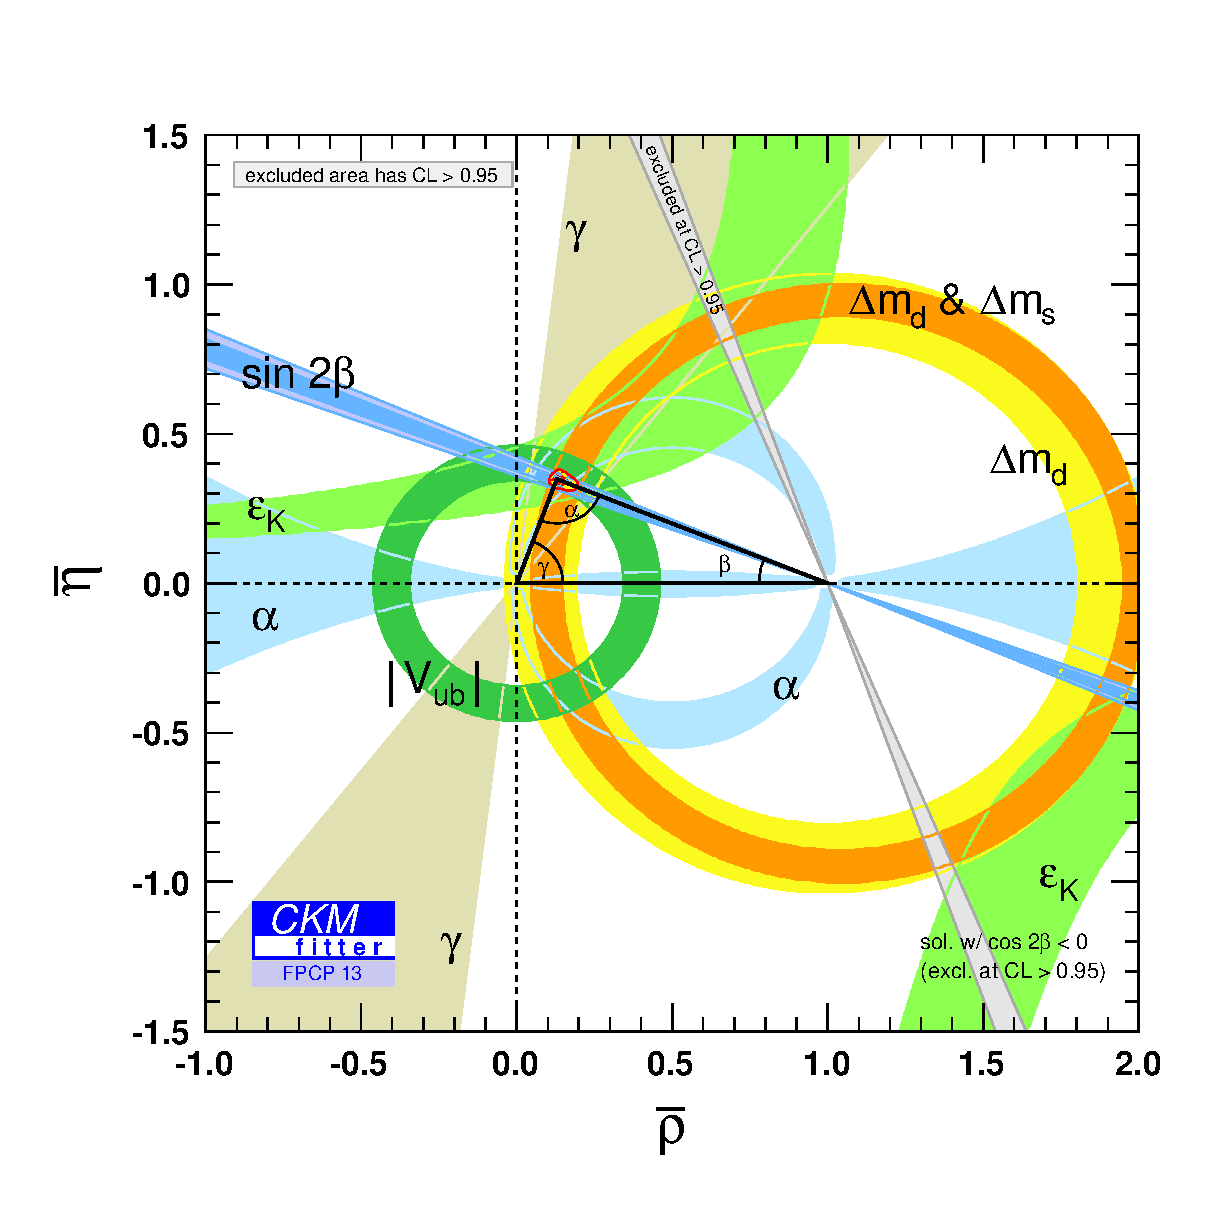
\includegraphics[width=0.55\linewidth]{ckm_triangle.eps}
%   \caption{Triangle d'unitarité de la matrice CKM. REFERENCE}
%   \label{fig:ckm_triangle}
% \end{figure}

\section{Conclusion}

On a vu au cours de ce chapitre comment a été construit le Modèle Standard. Fort de nombreuses prédictions et de la récente découverte d'un boson compatible avec le boson de Higgs par le CERN, le Modèle Standard est plus que jamais un succès théorique. Néanmoins, de nombreux arguments laissent penser que ce modèle n'est qu'une théorie effective d'une théorie plus simple et plus globale.

\bigskip

Il existe de nombreuses théories au-delà du Modèle Standard permettant de résoudre les faiblesses du modèle. Ces théories prédisent de nouvelles particules, de nouveaux bosons voire de nouvelles dimensions. Il est donc important pour les expérimentateurs de disposer d'outils adaptés permettant de vérifier les prédictions de ces nombreuses théories. C'est le cas du \emph{Large Hadron Collider} (\emph{LHC}, grand collisionneur de hadrons), dont la description détaillée est l'objet du prochain chapitre.

\end{fmffile}
